\section{Beamline geometry}

\subsection{The view from above}

If one were hovering above the beamline instrumentation with their head in the direction of the beam direction, then the forward direction is positive $z$, to the left is positive $x$, and the positive $y$ direction is upwards toward the sky. See diagram in Figure~\ref{fig_overview}. The coordinates of some main components are given in Figure~\ref{fig_coords}. Figure~\ref{fig_traj} shows an example trajectory of a particle through the beamline components.
\begin{figure}[h]	  
 \centering 
        	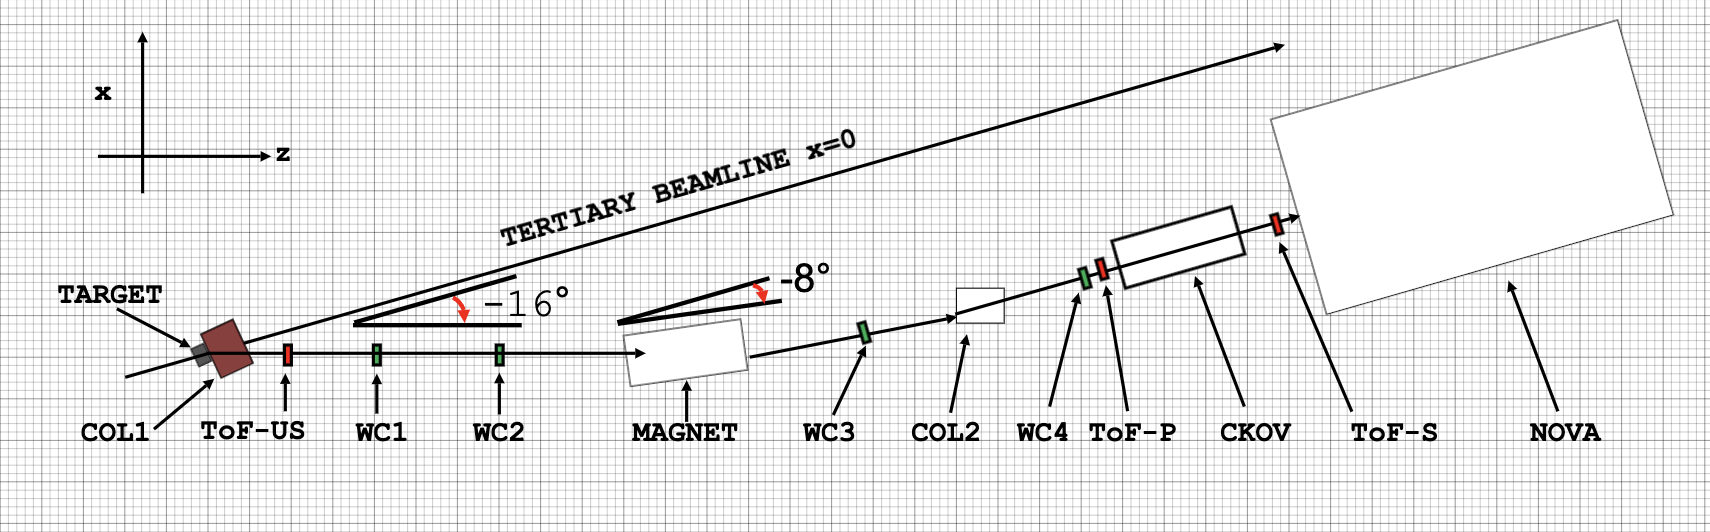
\includegraphics[scale=0.5]{overview.png}	 
   \caption[short]{A sketch of the beamline instrumentation as viewed from above.}
   \label{fig_overview}
  \end{figure}


% new table of coordinates
\begin{table}[ht]
\centering
%\begin{tabularx}{0.95\textwidth} { 
%   >{\raggedright\arraybackslash}X 
%  | >{\raggedleft\arraybackslash}X 
%  | >{\raggedleft\arraybackslash}X
%  | >{\raggedleft\arraybackslash}X
%  | >{\raggedleft\arraybackslash}X
%}
\begin{tabularx}{0.95\textwidth}{l | c | c | c | c}
\toprule
& \textbf{x [cm]} & \textbf{y[cm]} & z [cm] & $\theta$ [degrees] \\
\midrule
Target & 0.04 & -0.36 & 0.00 & 0\\
US Collimator  & 8.41 & -0.04  & 73.83 & -16\\
US ToF Period 3\&4 (2) & 40.58 (38.55) & -0.13 (0.75) & 141.57 (137.56) & -16\\
WC1 & -45.58 & 0.05 & 159.10 & -16\\
WC2 & -86.00 & 0.09 & 299.89 & -16 \\
Magnet & 129.7661 & -0.0254 & 472.8083 & -8\\

\bottomrule
\end{tabularx}
\caption{The positions of the centers of the beamline components, relative to a reference point close to the center of the target.}
\label{tab:coords}
\end{table}

There are three TOFs, all made of Lucite and having transverse size 5.91 square inches (15.01 cm). From thickest to thinnest they are 2.01cm, 1.32cm, 0.61cm. In period 2 the thickest one is used as the upstream ToF, and the thinnest one as the downstream PMT (Hamamatsu-H11934-200) ToF. These are switched for period 3 onwards. The 1.32cm thick ToF is read out by SensL C-series SiPM.

Particles produced by 64 GeV pions on the target have a chance of being detected if they make it through the acceptance of the upstream instrumentation. They must pass through the collimator, upstream ToF, and two wire chambers, and then impinge on the magnet fron face no more than 10cm from its center.

The aperture extent is 14.3 cm (x) by 5.2 cm (y). The ToF extent is 15.1 cm (x) by 15.1 cm (y).

The distance between the collimator aperture and the ToF is 67.7 cm.

The first wire chamber is 12.8 cm (x) by 12.8 cm (y) and is 17.5cm downstream of the ToF.

The second wire chamber is 12.8 cm (x) by 12.8 cm (y) and is 140.8cm downstream of the first wire chamber.

The constraining factor on tertiary beam particles is the second wire chamber.

The second wire chamber is 12.8 cm (x) by 12.8 cm (y) and is 226.0cm downstream of the collimator aperture. This puts a limit on the angle of deviation between the z-direction and the tertiary beam: $\pm 1.6^{\circ}$.

This is significantly smaller than the theoretically possible $\pm 3.6^{\circ}$ variation from z that is found from considering the dimensions of the collimator itself, 113.03cm (z) with US aperture size 7.11cm (x) by 5.2 cm (y) and DS aperture size twice the extent in x. Note that the $\pm 3.6^{\circ}$ is not an upeer limit - it assumes particles from the target enter the collimator at its transverse center. This approximation is also made in finding the $\pm 1.6^{\circ}$.

Extrapolating this $\pm 1.6^{\circ}$ constraint to the front face of the magnet, which is 399.0 cm from the collimator aperture, gives x = ztanbeta = 11.3 cm.

The angular spread in y from the collimator is $\pm 1.3^{\circ}$; this is slightly less than the WC2 constraint, and so we expect and observe a slightly more condensed angular distribution in y when looking at wire chamber hit distributions. 

The magnet is 76.2 cm (y) by 106.7 cm (z) by 127 cm (x).

The field region is 8.9 cm (y) by 106.7 cm (z) by 45.1 cm (x). I don't think this is correct for x. It looks like from \href{https://nova-docdb.fnal.gov/cgi-bin/sso/RetrieveFile?docid=46939&filename=testbeam-analysis-bfield.pdf&version=1}{Mark's slides} that the effective field in x is from +/10 cm, with stability in +/-8cm.






\begin{figure}[h]	   
 \centering
        	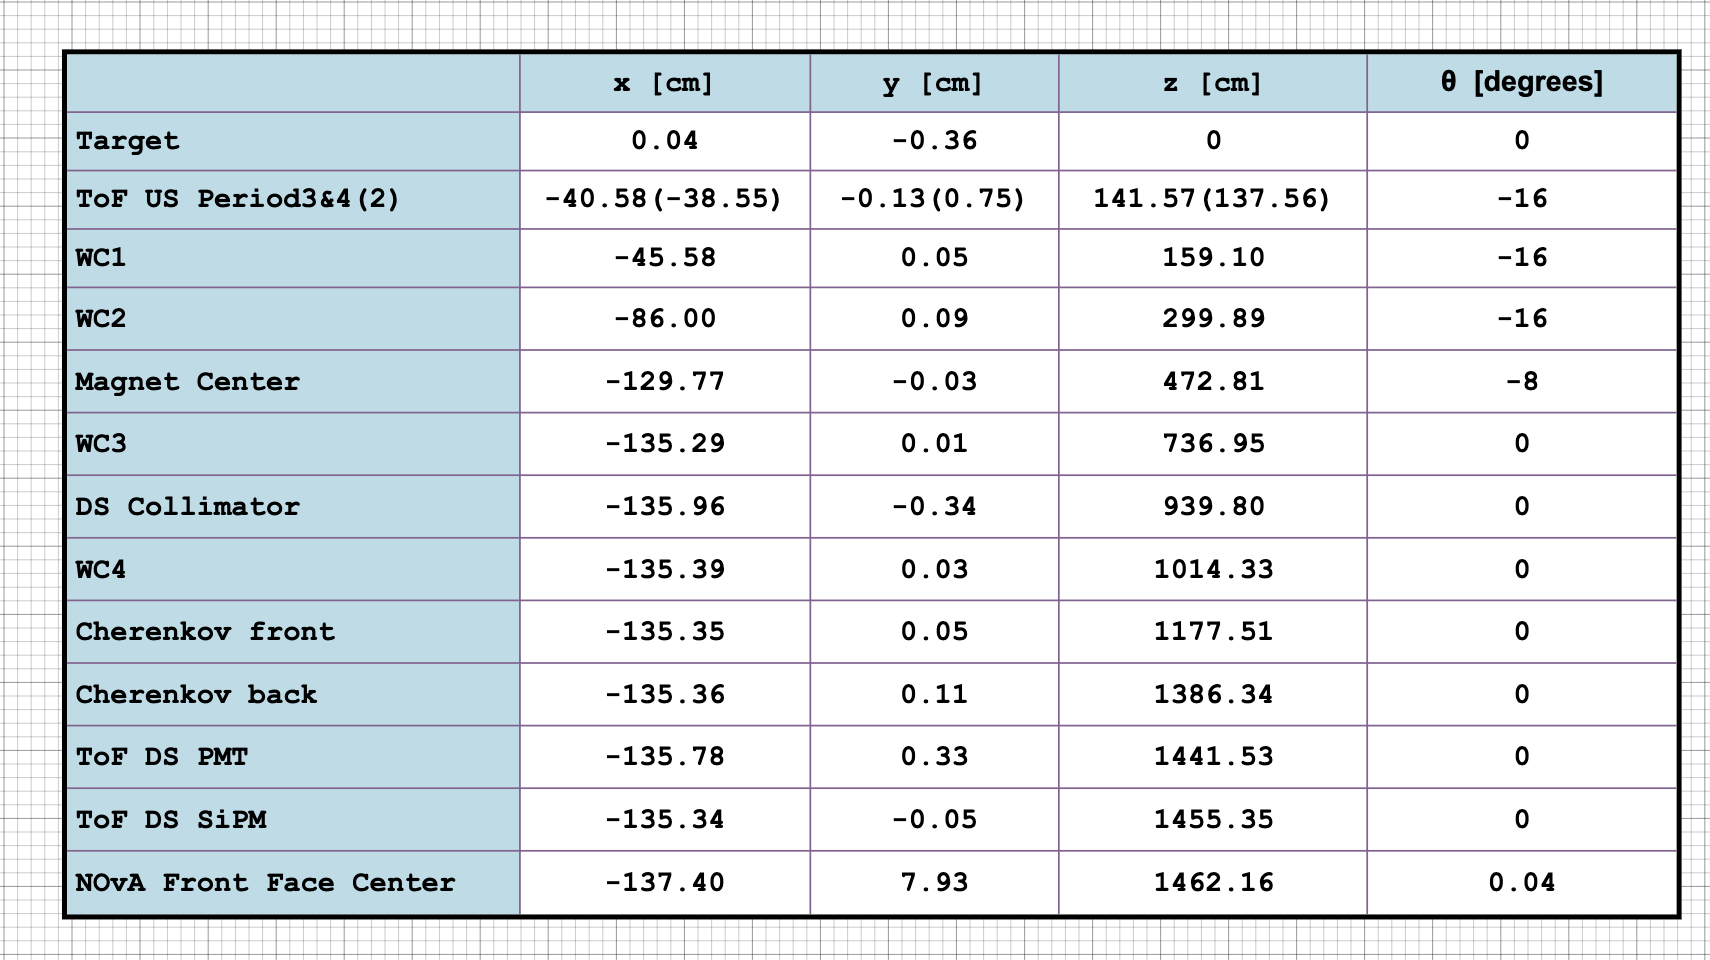
\includegraphics[scale=0.5]{coords.png}	 
   \caption[short]{Coordinates of some of the main components of the beamline instrumentation.}
   \label{fig_coords}
  \end{figure}
  
    \begin{figure}[h]	   
 \centering
        	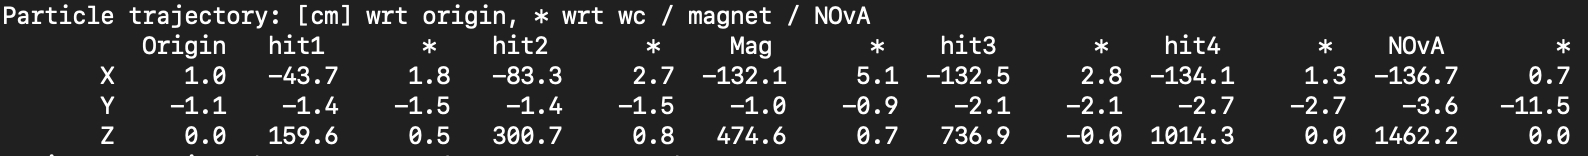
\includegraphics[scale=0.5]{example-traj.png}	 
   \caption[short]{An example trajectory of measurements along the beamline.}
   \label{fig_traj}
  \end{figure}
  
  
\subsection{The wirechamber coordinates}

Figure~\ref{fig_xyhits} show the hit positions in the four wirechambers. \textcolor{red}{The missing wires in WC1 increase over the periods of data taking, shown in Figure~\ref{fig_xyhitsperiod}}.

       \begin{figure}[h]	   
            \centering
   
            \begin{subfigure}[b]{0.23\textwidth}
            \centering
            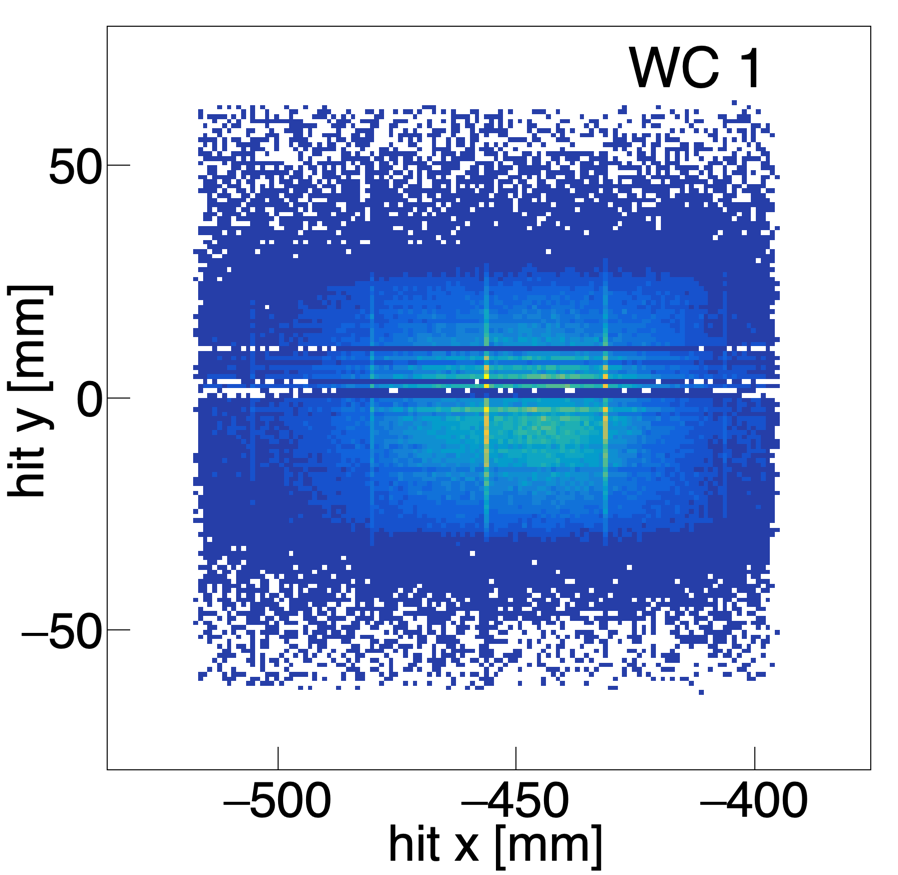
\includegraphics[width=\textwidth]{wcn_xy1_pol-1_period234_miss0.png}
            \caption{WC1}
            \label{fig_wc1}
            \end{subfigure}
            \hfill             
             \begin{subfigure}[b]{0.23\textwidth}
            \centering
            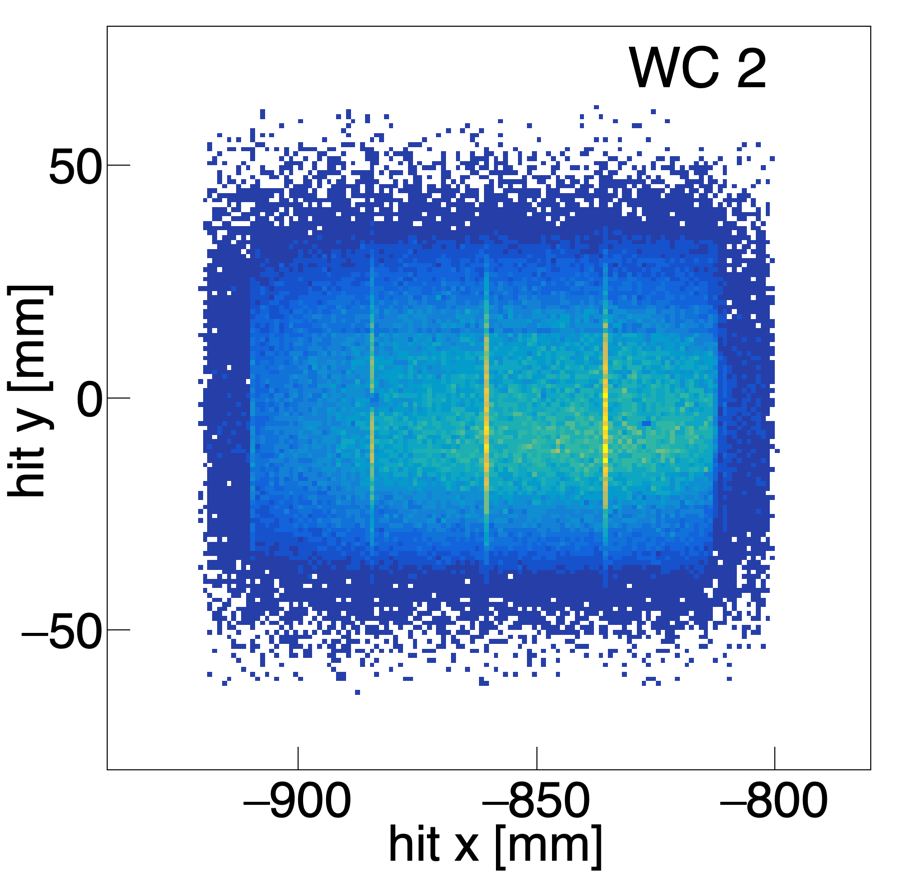
\includegraphics[width=\textwidth]{wcn_xy2_pol-1_period234_miss0.png}
            \caption{WC2}
            \label{fig_wc2}
            \end{subfigure}
            \hfill 
              \begin{subfigure}[b]{0.23\textwidth}
            \centering
            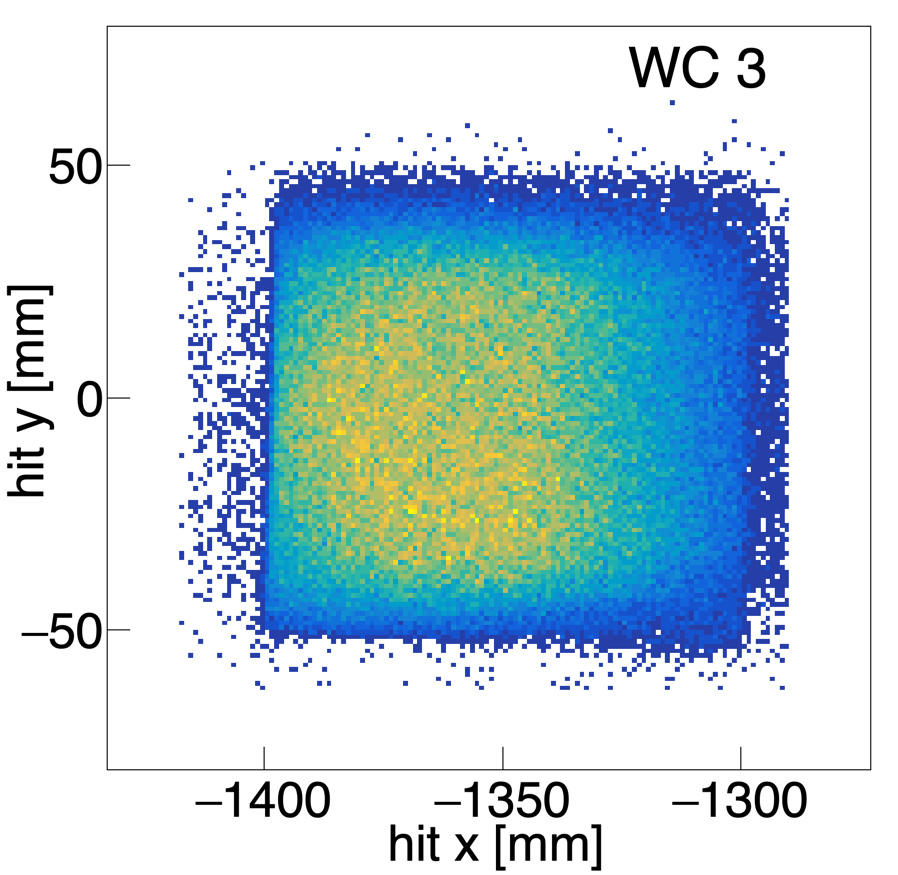
\includegraphics[width=\textwidth]{wcn_xy3_pol-1_period234_miss0.png}
            \caption{WC3}
            \label{fig_wc3}
            \end{subfigure}
            \hfill    
             \begin{subfigure}[b]{0.23\textwidth}
            \centering
            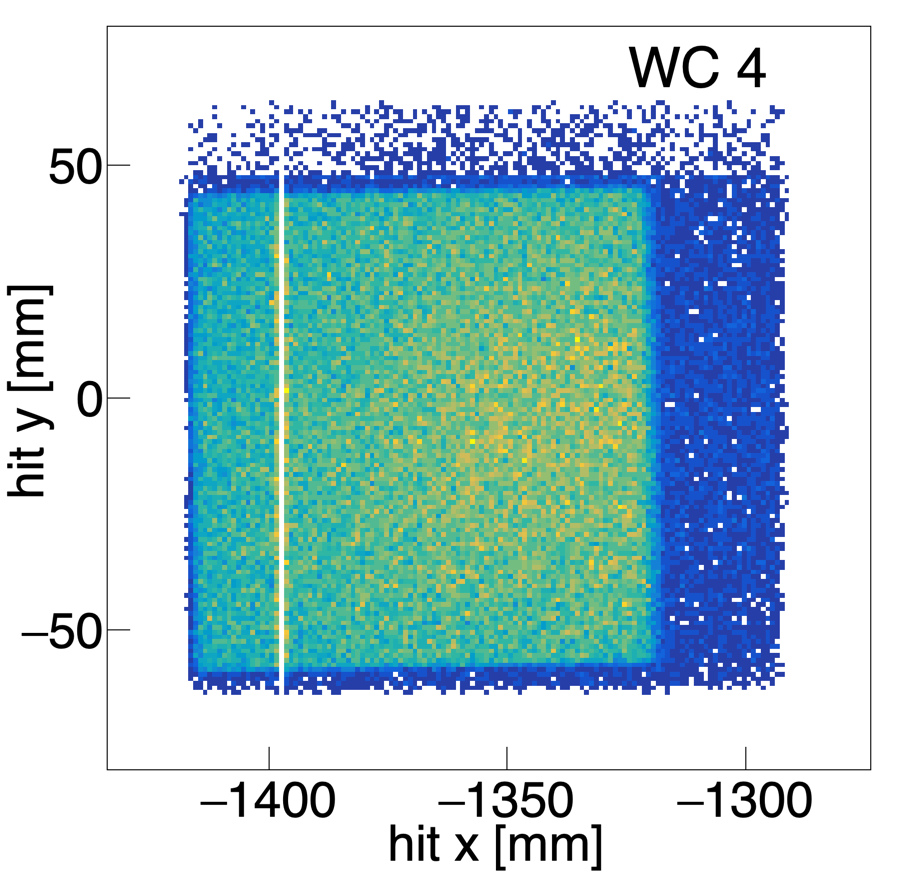
\includegraphics[width=\textwidth]{wcn_xy4_pol-1_period234_miss0.png}
            \caption{WC4}
            \label{fig_wc4}
            \end{subfigure}
            \hfill
   \caption[short]{The WCTrack best hit position in each of the four wire chambers, relative to the collimated tertiary beam. The best hit here means the hit that was attributed to the best track fit. Notice that wire chamber 1 has missing wires. All four hits must be present for these plots to be filled}
   \label{fig_xyhits}
  \end{figure}
  
  
         \begin{figure}[h]	   
            \centering
   	%miss 2
            \begin{subfigure}[b]{0.23\textwidth}
            \centering
            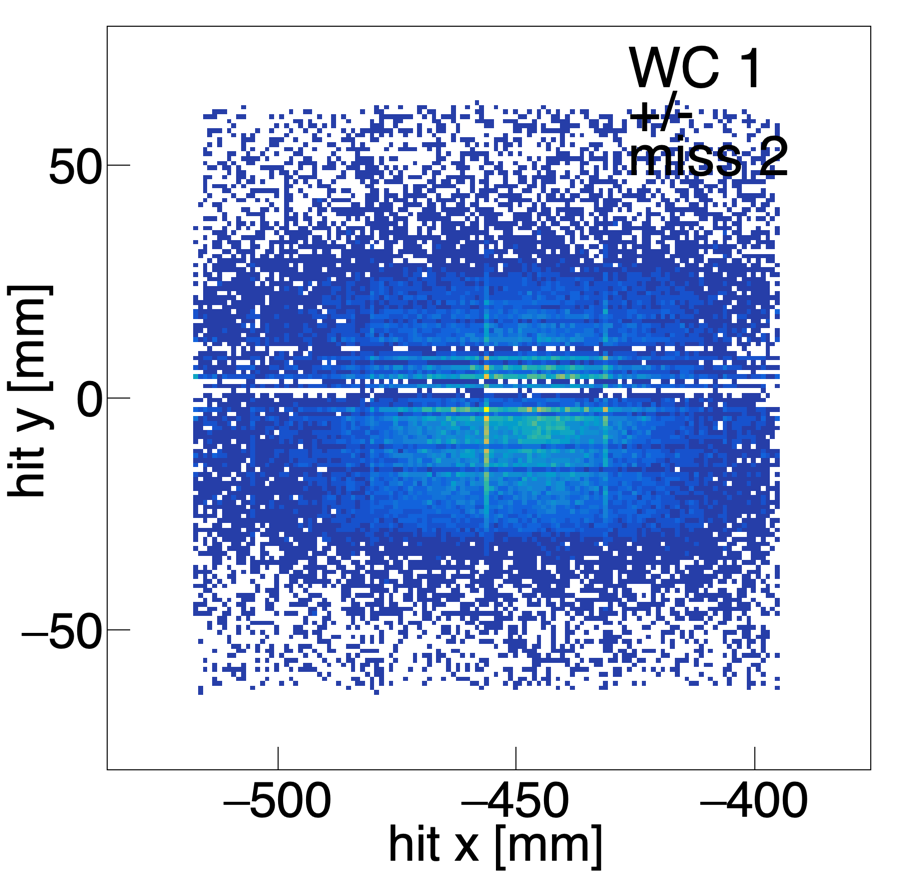
\includegraphics[width=\textwidth]{wcn_xy1_pol-1_period234_miss2.png}
            \caption{WC1, miss2}
            \label{fig_wc1}
            \end{subfigure}
            \hfill             
             \begin{subfigure}[b]{0.23\textwidth}
            \centering
            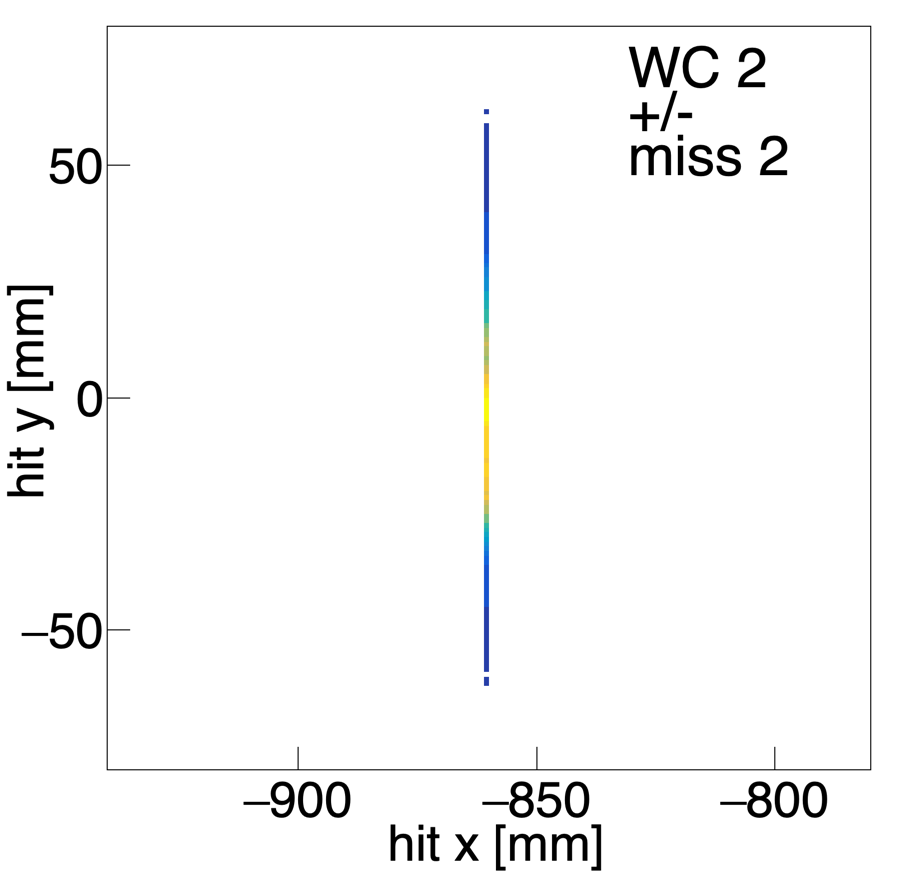
\includegraphics[width=\textwidth]{wcn_xy2_pol-1_period234_miss2.png}
            \caption{WC2, miss2}
            \label{fig_wc2}
            \end{subfigure}
            \hfill 
              \begin{subfigure}[b]{0.23\textwidth}
            \centering
            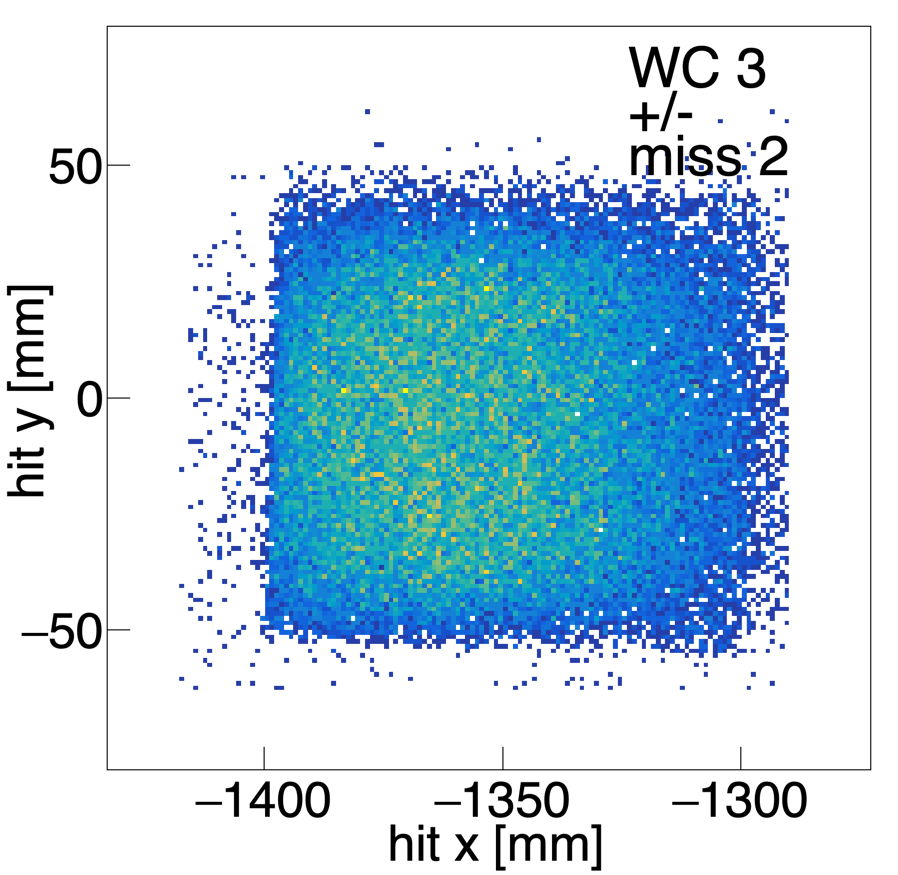
\includegraphics[width=\textwidth]{wcn_xy3_pol-1_period234_miss2.png}
            \caption{WC3, miss2}
            \label{fig_wc3}
            \end{subfigure}
            \hfill    
             \begin{subfigure}[b]{0.23\textwidth}
            \centering
            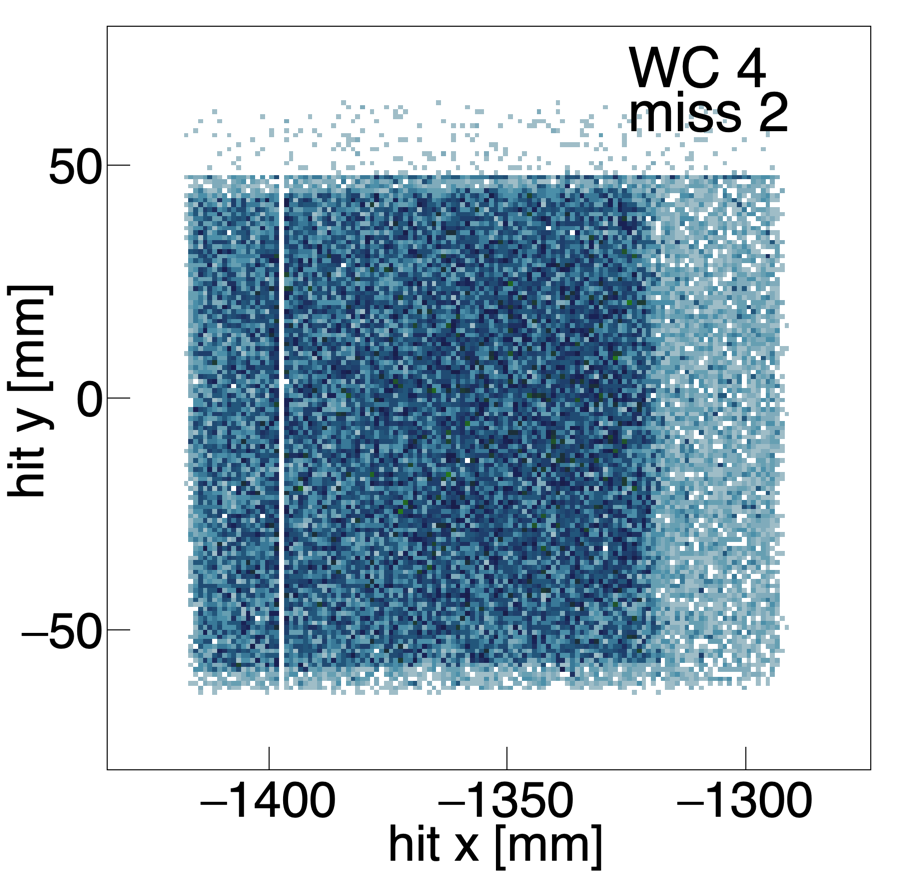
\includegraphics[width=\textwidth]{wcn_xy4_pol-1_period234_miss2.png}
            \caption{WC4, miss2}
            \label{fig_wc4}
            \end{subfigure}
            \hfill
            %miss3
                     \begin{subfigure}[b]{0.23\textwidth}
            \centering
            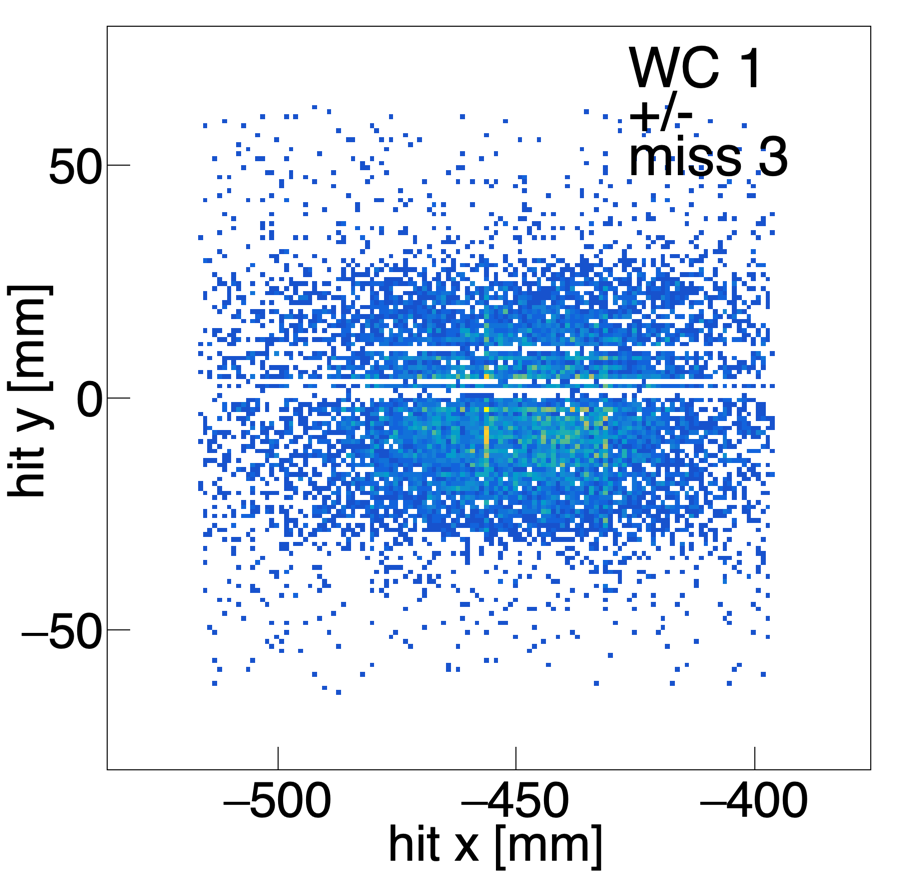
\includegraphics[width=\textwidth]{wcn_xy1_pol-1_period234_miss3.png}
            \caption{WC1, miss3}
            \label{fig_wc1}
            \end{subfigure}
            \hfill             
             \begin{subfigure}[b]{0.23\textwidth}
            \centering
            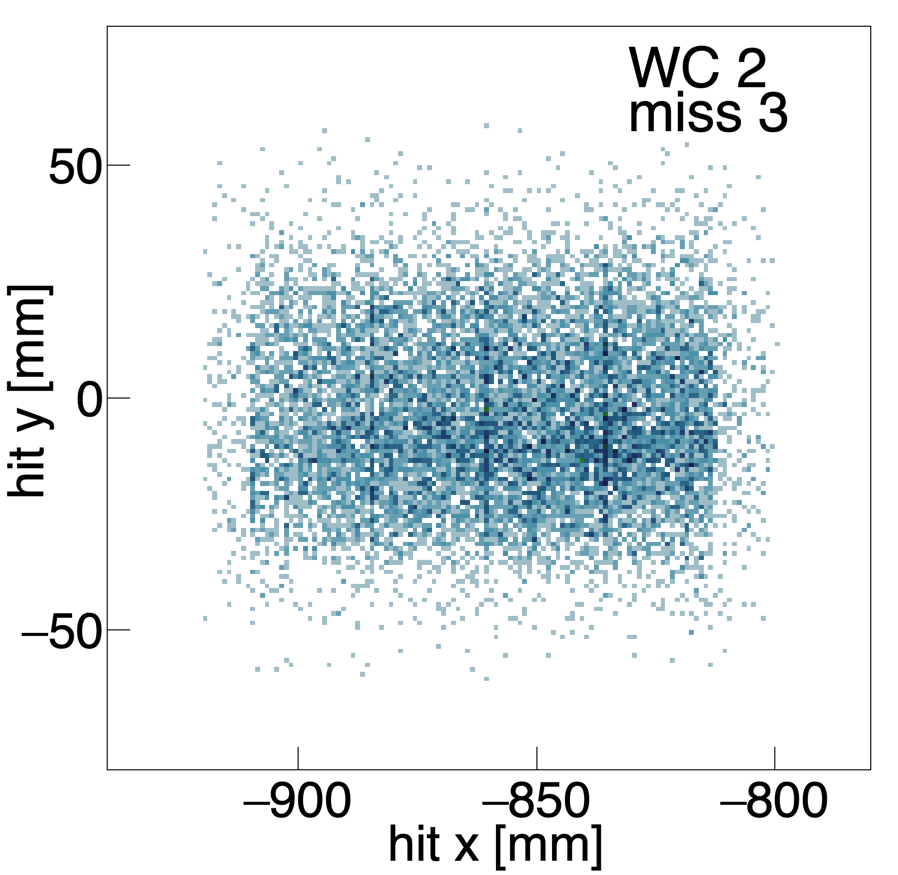
\includegraphics[width=\textwidth]{wcn_xy2_pol-1_period234_miss3.png}
            \caption{WC2, miss3}
            \label{fig_wc2}
            \end{subfigure}
            \hfill 
              \begin{subfigure}[b]{0.23\textwidth}
            \centering
            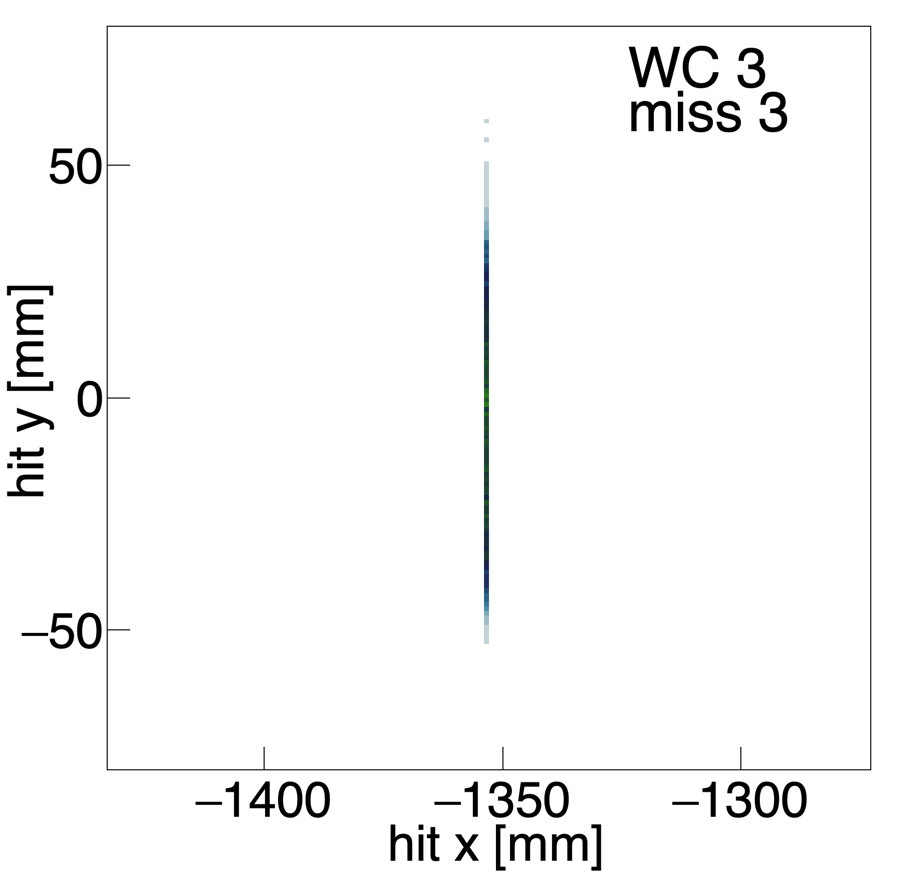
\includegraphics[width=\textwidth]{wcn_xy3_pol-1_period234_miss3.png}
            \caption{WC3, miss3}
            \label{fig_wc3}
            \end{subfigure}
            \hfill    
             \begin{subfigure}[b]{0.23\textwidth}
            \centering
            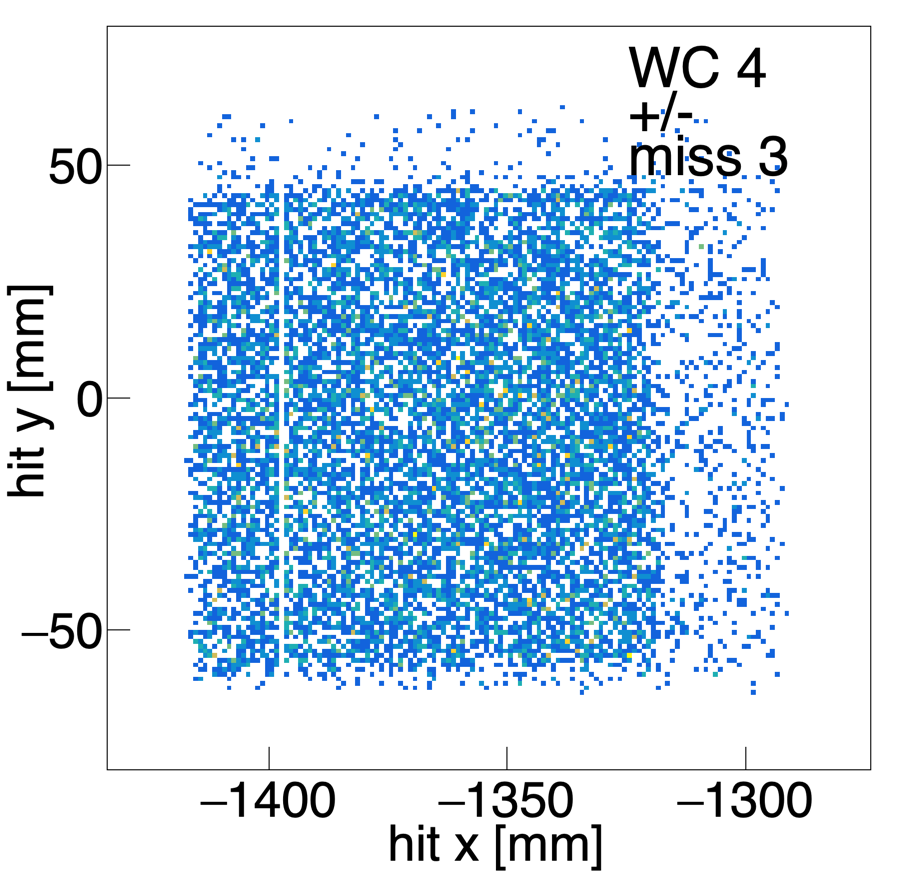
\includegraphics[width=\textwidth]{wcn_xy4_pol-1_period234_miss3.png}
            \caption{WC4, miss3}
            \label{fig_wc4}
            \end{subfigure}
            \hfill
            
             %miss3
                     \begin{subfigure}[b]{0.23\textwidth}
            \centering
            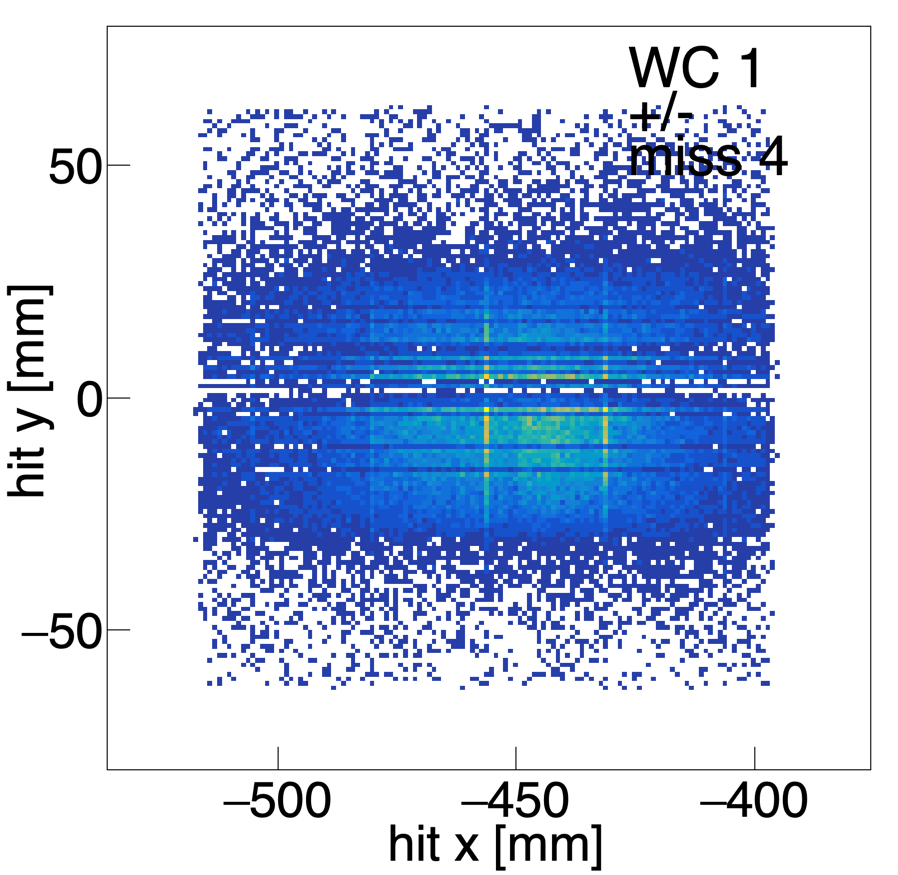
\includegraphics[width=\textwidth]{wcn_xy1_pol-1_period234_miss4.png}
            \caption{WC1, miss4}
            \label{fig_wc1}
            \end{subfigure}
            \hfill             
             \begin{subfigure}[b]{0.23\textwidth}
            \centering
            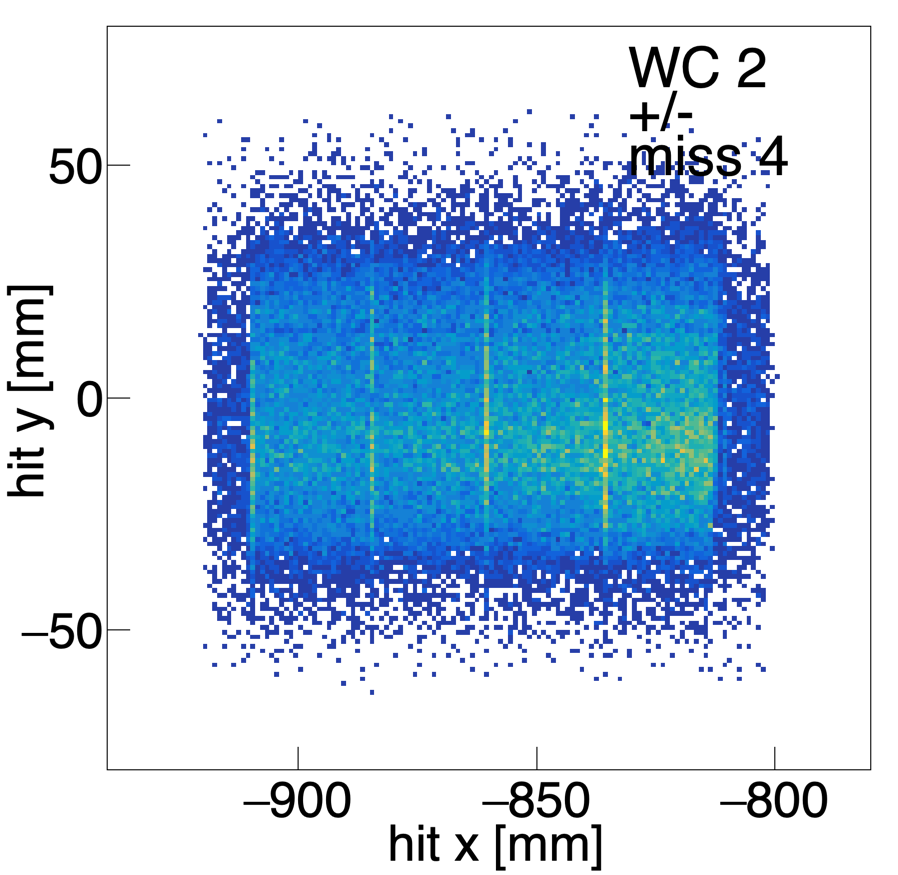
\includegraphics[width=\textwidth]{wcn_xy2_pol-1_period234_miss4.png}
            \caption{WC2, miss4}
            \label{fig_wc2}
            \end{subfigure}
            \hfill 
              \begin{subfigure}[b]{0.23\textwidth}
            \centering
            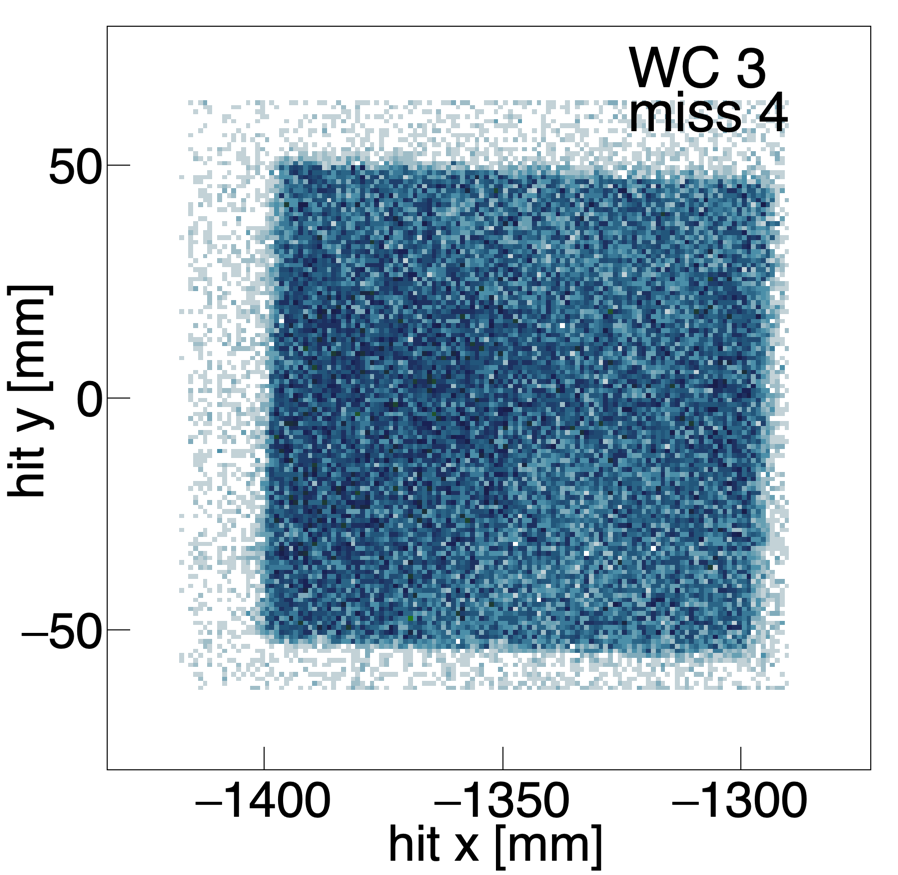
\includegraphics[width=\textwidth]{wcn_xy3_pol-1_period234_miss4.png}
            \caption{WC3, miss4}
            \label{fig_wc3}
            \end{subfigure}
            \hfill    
             \begin{subfigure}[b]{0.23\textwidth}
            \centering
            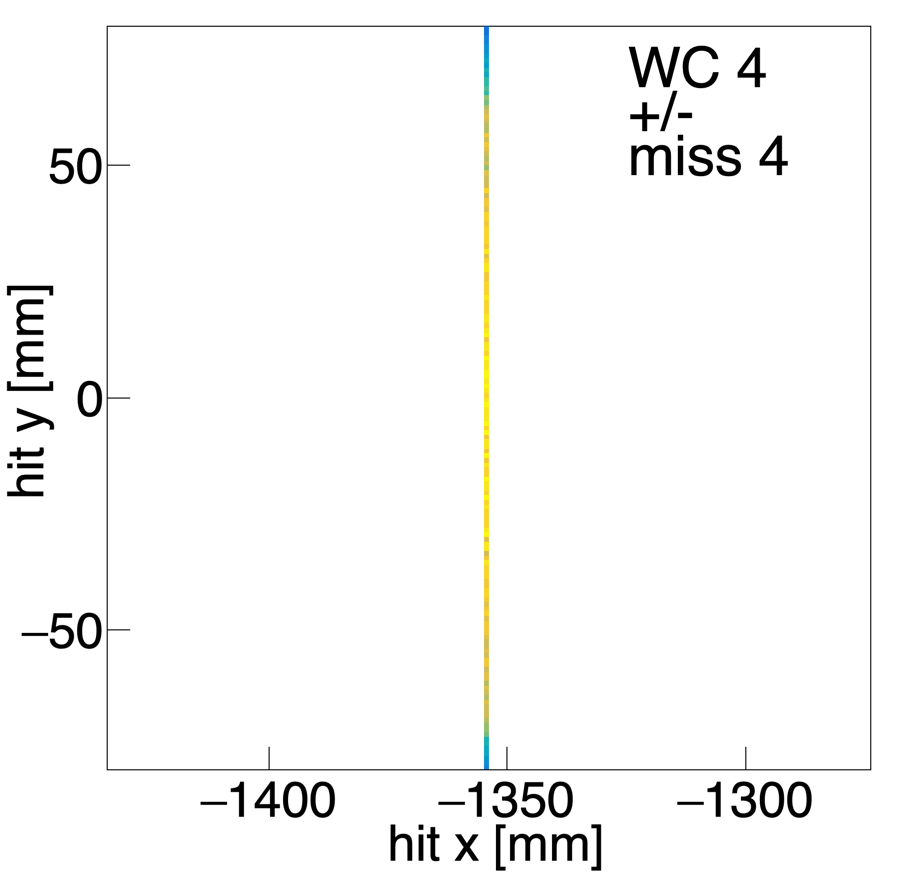
\includegraphics[width=\textwidth]{wcn_xy4_pol-1_period234_miss4.png}
            \caption{WC4, miss4}
            \label{fig_wc4}
            \end{subfigure}
            \hfill

   \caption[short]{The WCTrack best hit position in each of the four wire chambers, relative to the collimated tertiary beam. The best hit here means the hit that was attributed to the best track fit. Notice that wire chamber 1 has missing wires. Top row: tracks where the hit in wc2 is faked, middle row: hit 2 is faked, bottom row: hit 4 is faked.}
   \label{fig_xyhits}
  \end{figure}
  
  
  
  
  
         \begin{figure}[h]	   
            \centering
   
               \begin{subfigure}[b]{0.23\textwidth}
            \centering
            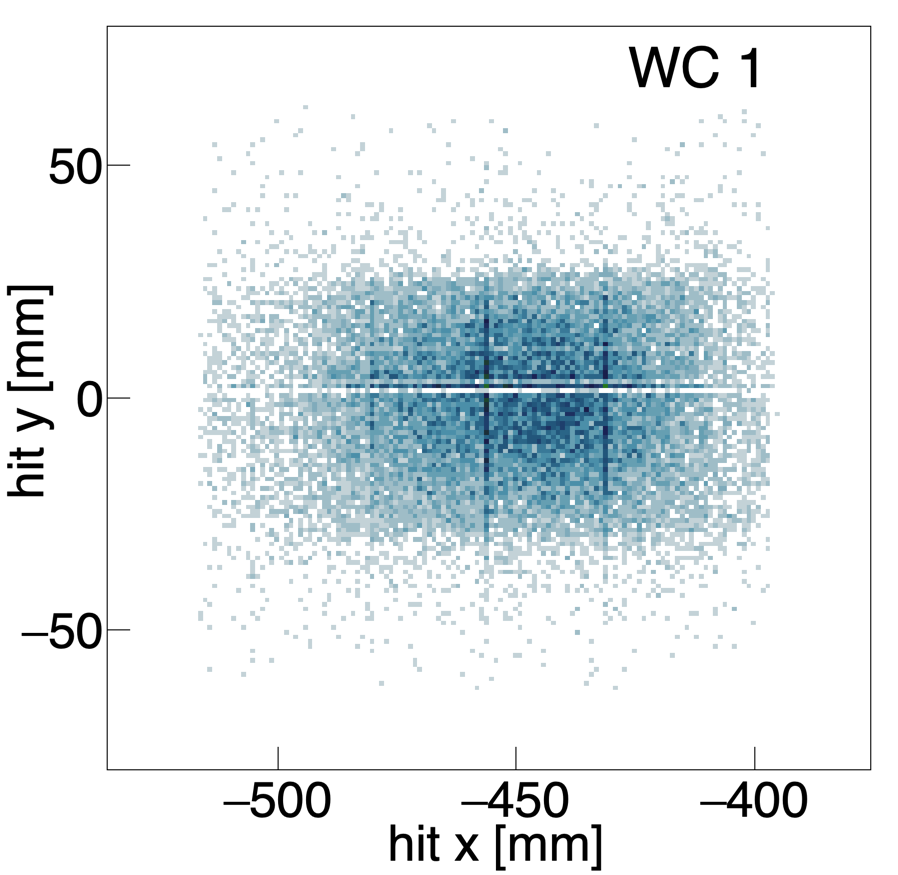
\includegraphics[width=\textwidth]{wcn_xy1_pol-1_period2_miss0.png}
            \caption{WC1, P2}
            \label{fig_wc1_p2}
            \end{subfigure}
            \hfill             
             \begin{subfigure}[b]{0.23\textwidth}
            \centering
            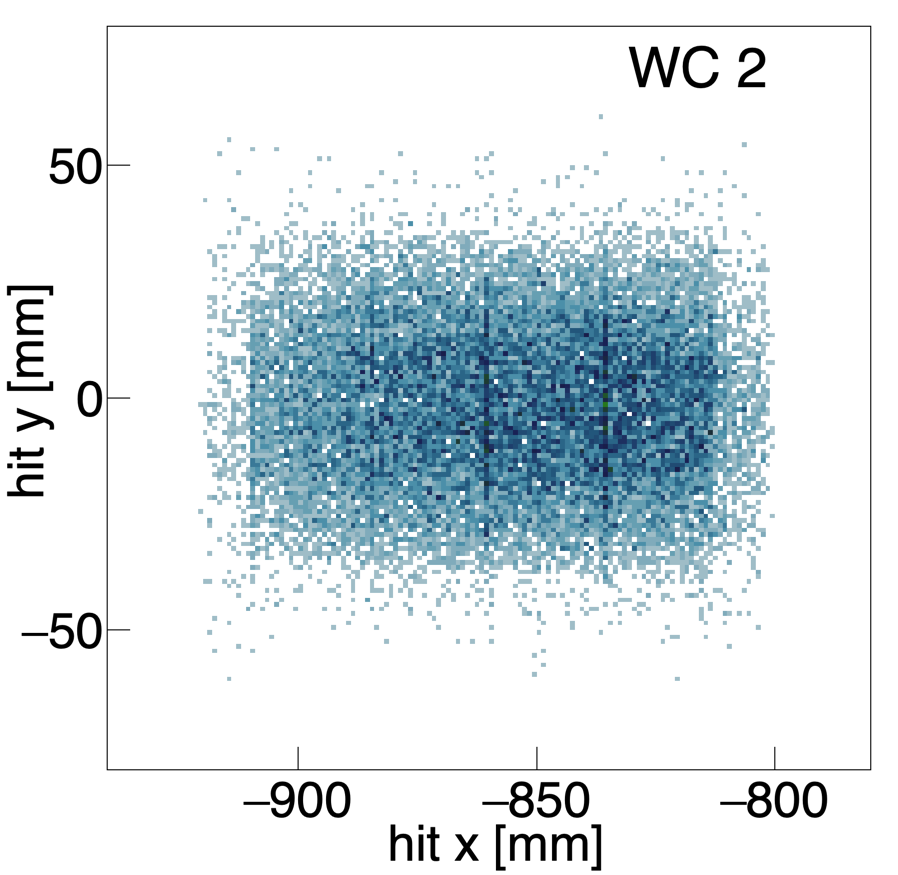
\includegraphics[width=\textwidth]{wcn_xy2_pol-1_period2_miss0.png}
            \caption{WC2, P2}
            \label{fig_wc2_p2}
            \end{subfigure}
            \hfill 
              \begin{subfigure}[b]{0.23\textwidth}
            \centering
            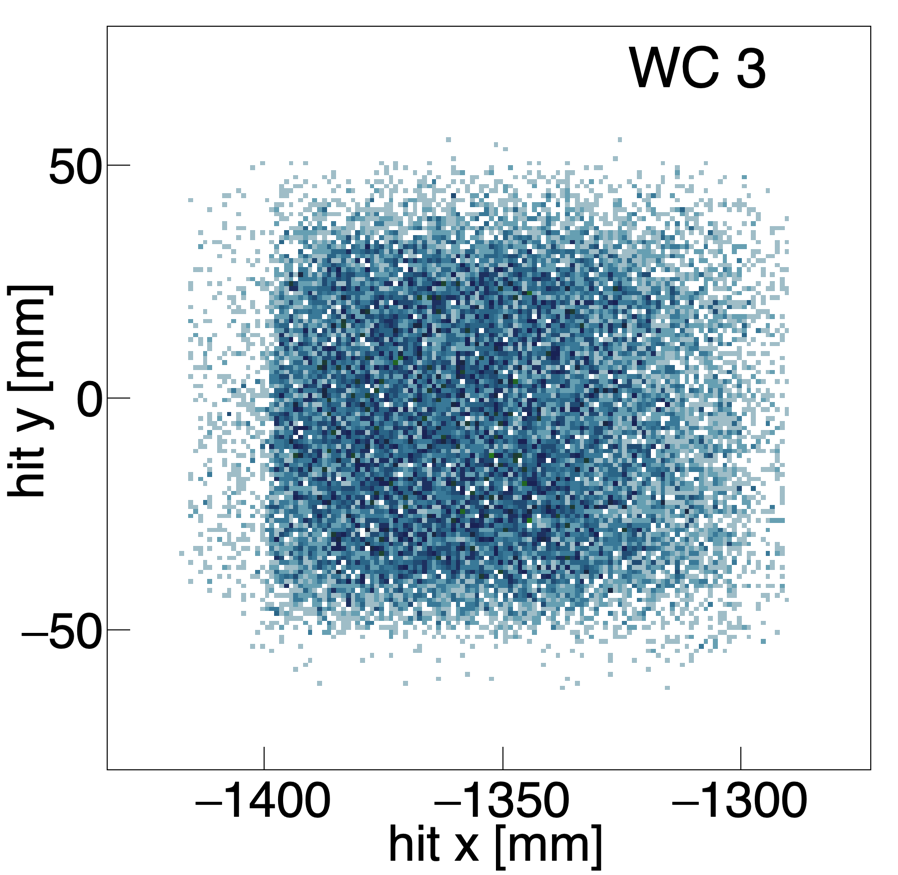
\includegraphics[width=\textwidth]{wcn_xy3_pol-1_period2_miss0.png}
            \caption{WC3, P2}
            \label{fig_wc3_p2}
            \end{subfigure}
            \hfill    
             \begin{subfigure}[b]{0.23\textwidth}
            \centering
            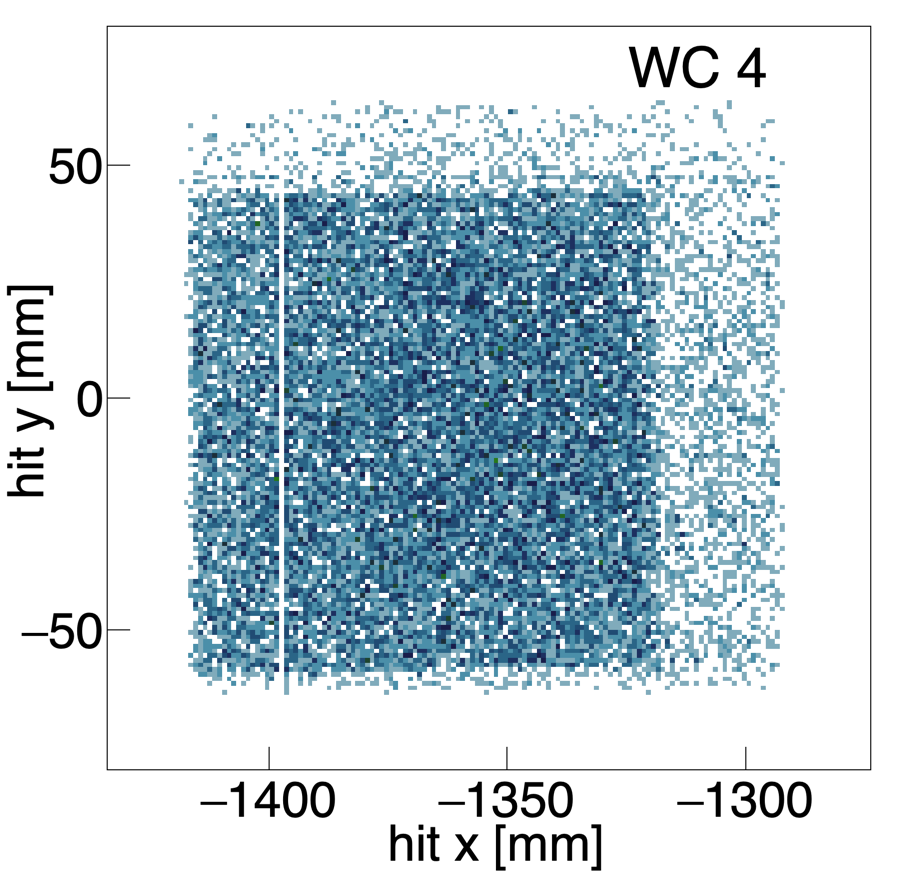
\includegraphics[width=\textwidth]{wcn_xy4_pol-1_period2_miss0.png}
            \caption{WC4, P2}
            \label{fig_wc4_p2}
            \end{subfigure}
            \hfill
   %p3
               \begin{subfigure}[b]{0.23\textwidth}
            \centering
            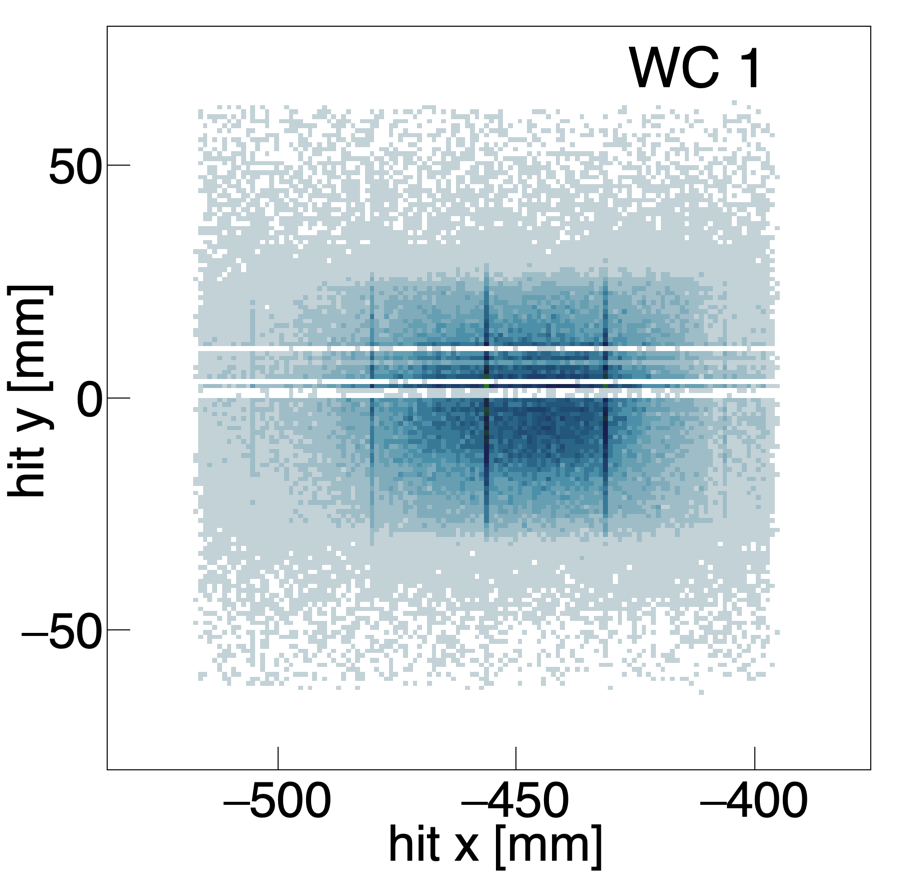
\includegraphics[width=\textwidth]{wcn_xy1_pol-1_period3_miss0.png}
            \caption{WC1, P3}
            \label{fig_wc1_p3}
            \end{subfigure}
            \hfill             
             \begin{subfigure}[b]{0.23\textwidth}
            \centering
            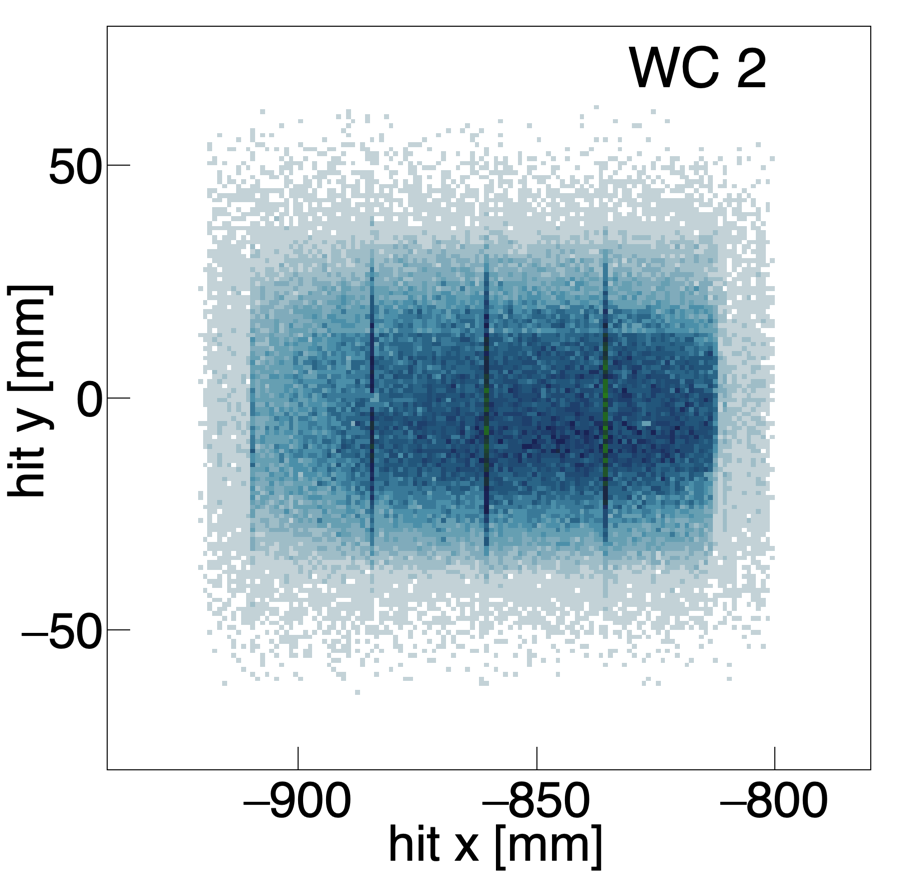
\includegraphics[width=\textwidth]{wcn_xy2_pol-1_period3_miss0.png}
            \caption{WC2, P3}
            \label{fig_wc2_p3}
            \end{subfigure}
            \hfill 
              \begin{subfigure}[b]{0.23\textwidth}
            \centering
            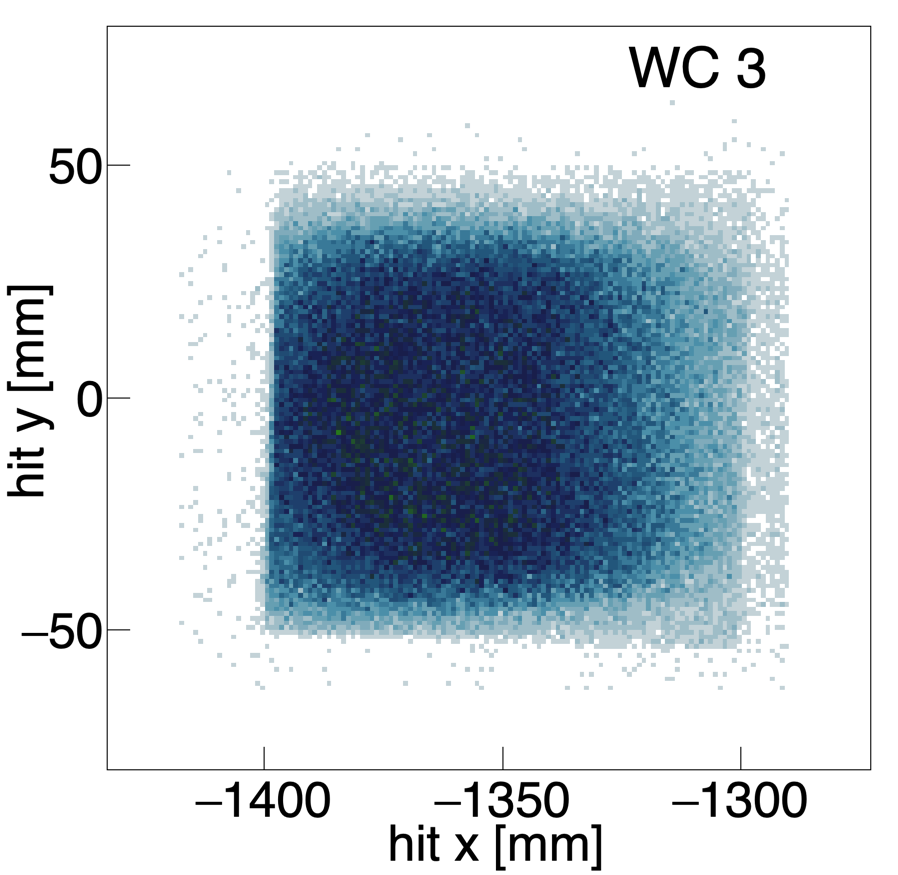
\includegraphics[width=\textwidth]{wcn_xy3_pol-1_period3_miss0.png}
            \caption{WC3, P3}
            \label{fig_wc3_p3}
            \end{subfigure}
            \hfill    
             \begin{subfigure}[b]{0.23\textwidth}
            \centering
            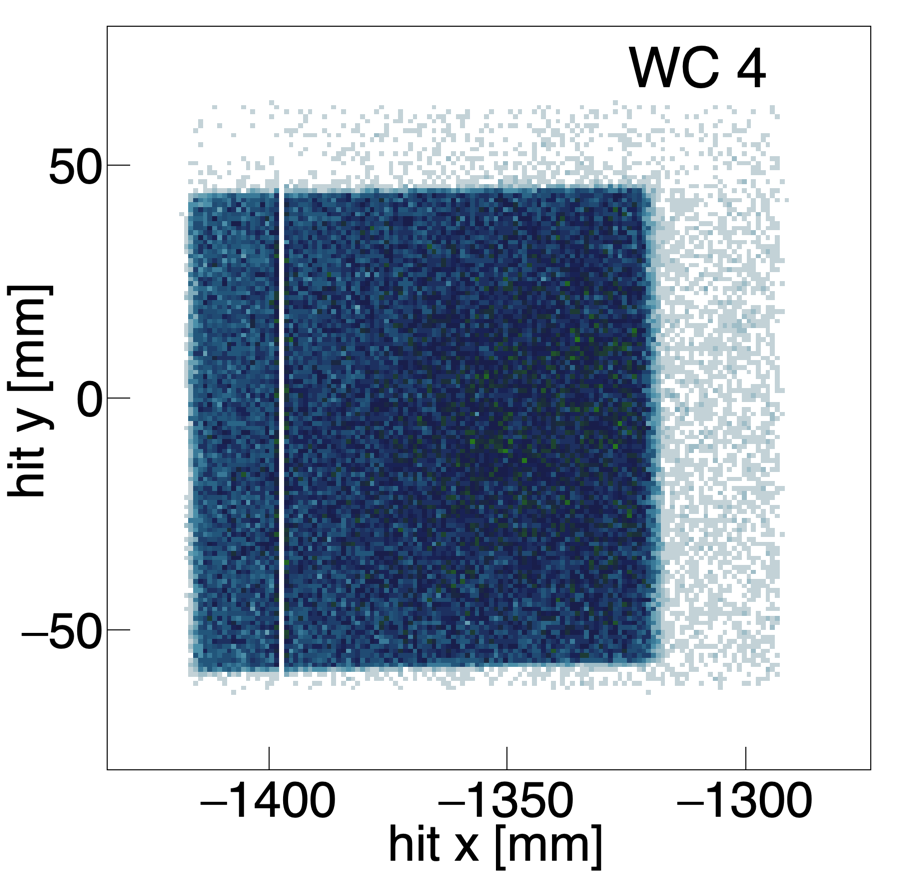
\includegraphics[width=\textwidth]{wcn_xy4_pol-1_period3_miss0.png}
            \caption{WC4, P3}
            \label{fig_wc4_p3}
            \end{subfigure}
            \hfill
   %p4
            \begin{subfigure}[b]{0.23\textwidth}
            \centering
            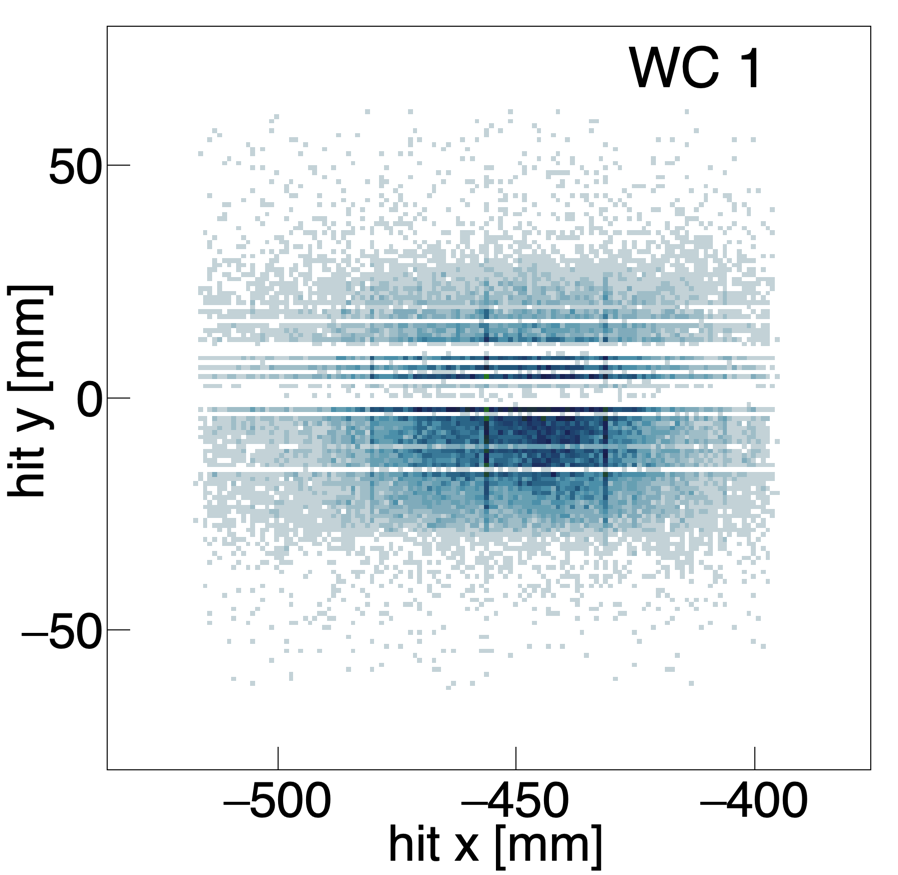
\includegraphics[width=\textwidth]{wcn_xy1_pol-1_period4_miss0.png}
            \caption{WC1, P4}
            \label{fig_wc1_p4}
            \end{subfigure}
            \hfill             
             \begin{subfigure}[b]{0.23\textwidth}
            \centering
            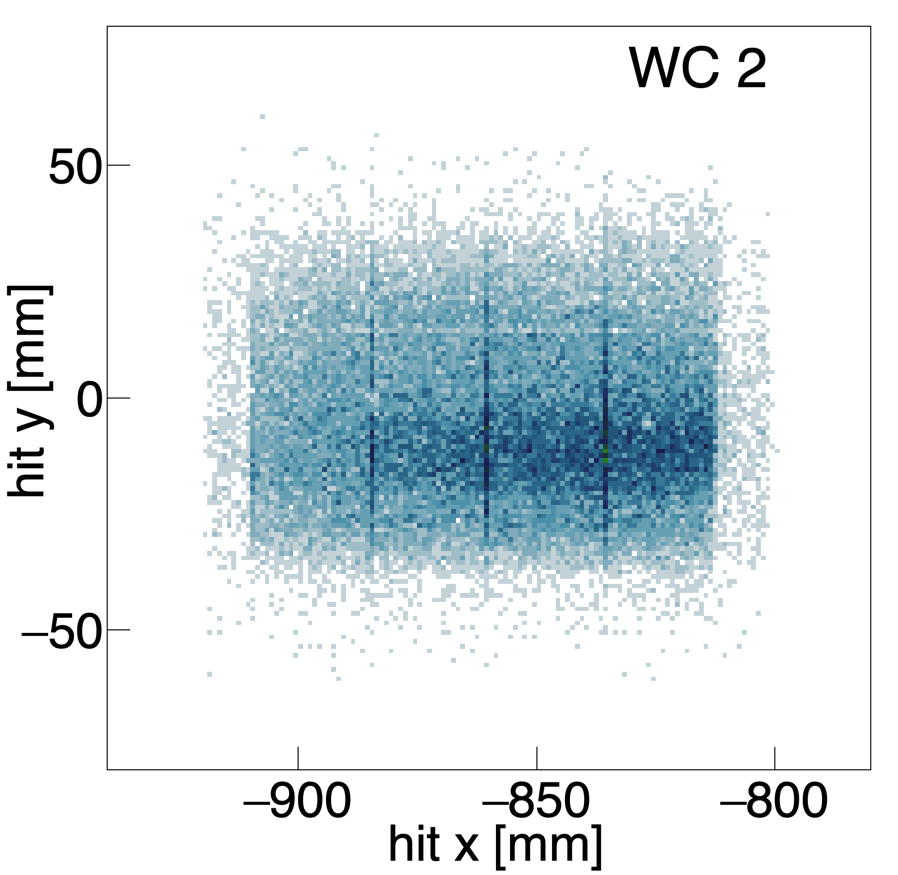
\includegraphics[width=\textwidth]{wcn_xy2_pol-1_period4_miss0.png}
            \caption{WC2, P4}
            \label{fig_wc2_p4}
            \end{subfigure}
            \hfill 
              \begin{subfigure}[b]{0.23\textwidth}
            \centering
            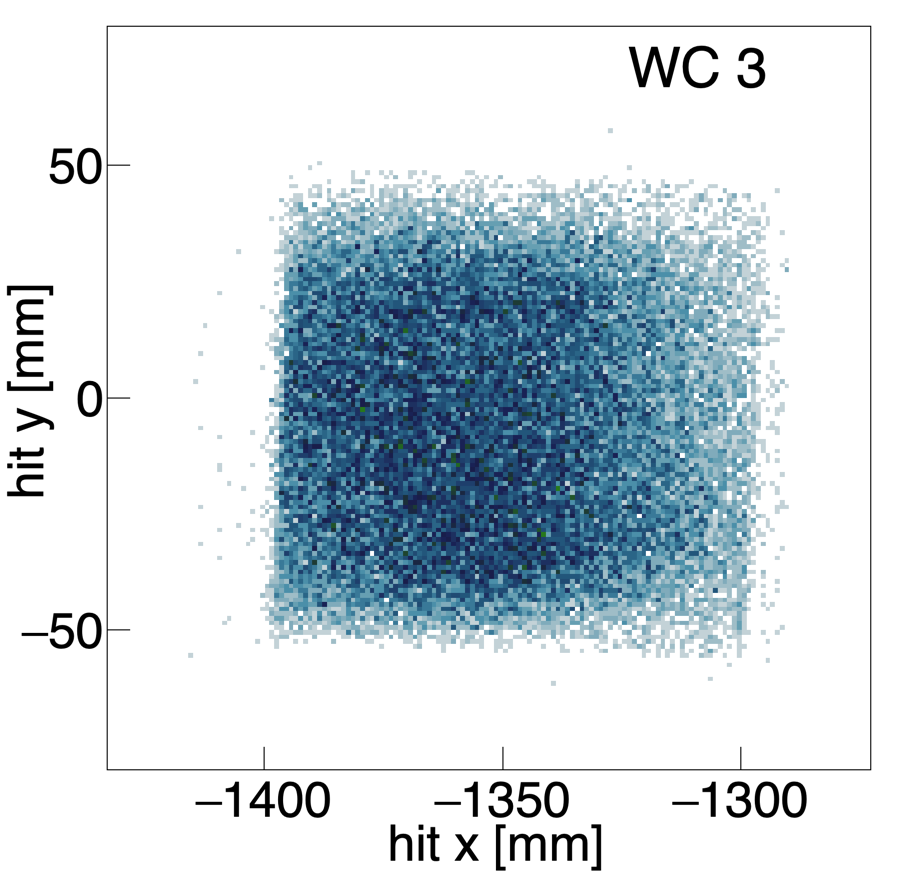
\includegraphics[width=\textwidth]{wcn_xy3_pol-1_period4_miss0.png}
            \caption{WC3, P4}
            \label{fig_wc3_p4}
            \end{subfigure}
            \hfill    
             \begin{subfigure}[b]{0.23\textwidth}
            \centering
            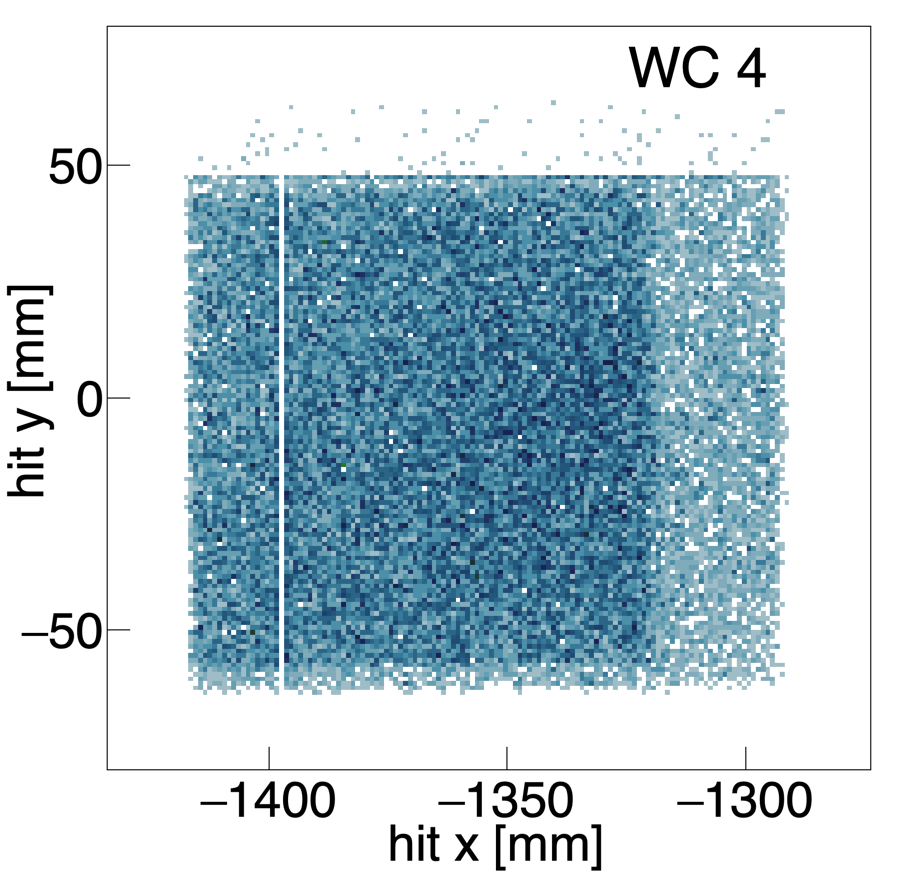
\includegraphics[width=\textwidth]{wcn_xy4_pol-1_period4_miss0.png}
            \caption{WC4, P4}
            \label{fig_wc4_p4}
            \end{subfigure}
            \hfill
   \caption[short]{The WCTrack best hit position in each of the four wire chambers, divided by period.}
   \label{fig_xyhitsperiod}
  \end{figure}
  
  
  
           \begin{figure}[h]	   
            \centering
   
               \begin{subfigure}[b]{0.23\textwidth}
            \centering
            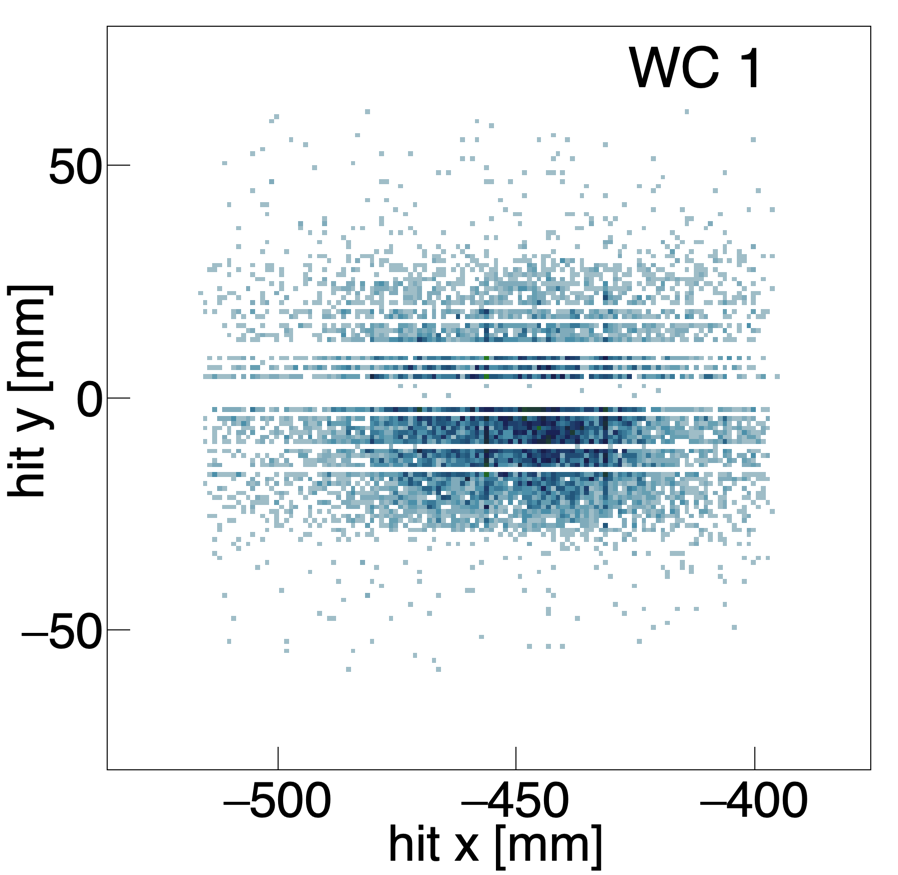
\includegraphics[width=\textwidth]{wcn_xy1_pol0_period4_miss0.png}
            \caption{WC1, P3}
            \label{fig_wc1_p3}
            \end{subfigure}
            \hfill             
             \begin{subfigure}[b]{0.23\textwidth}
            \centering
            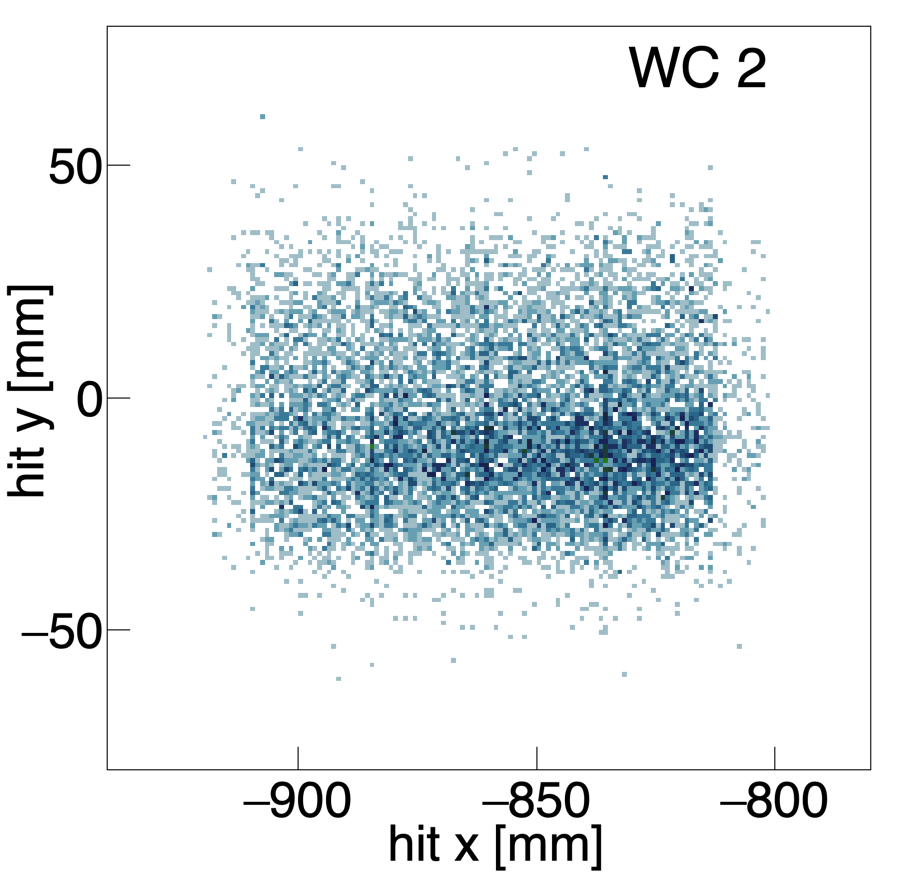
\includegraphics[width=\textwidth]{wcn_xy2_pol0_period4_miss0.png}
            \caption{WC2, P3}
            \label{fig_wc2_p3}
            \end{subfigure}
            \hfill 
              \begin{subfigure}[b]{0.23\textwidth}
            \centering
            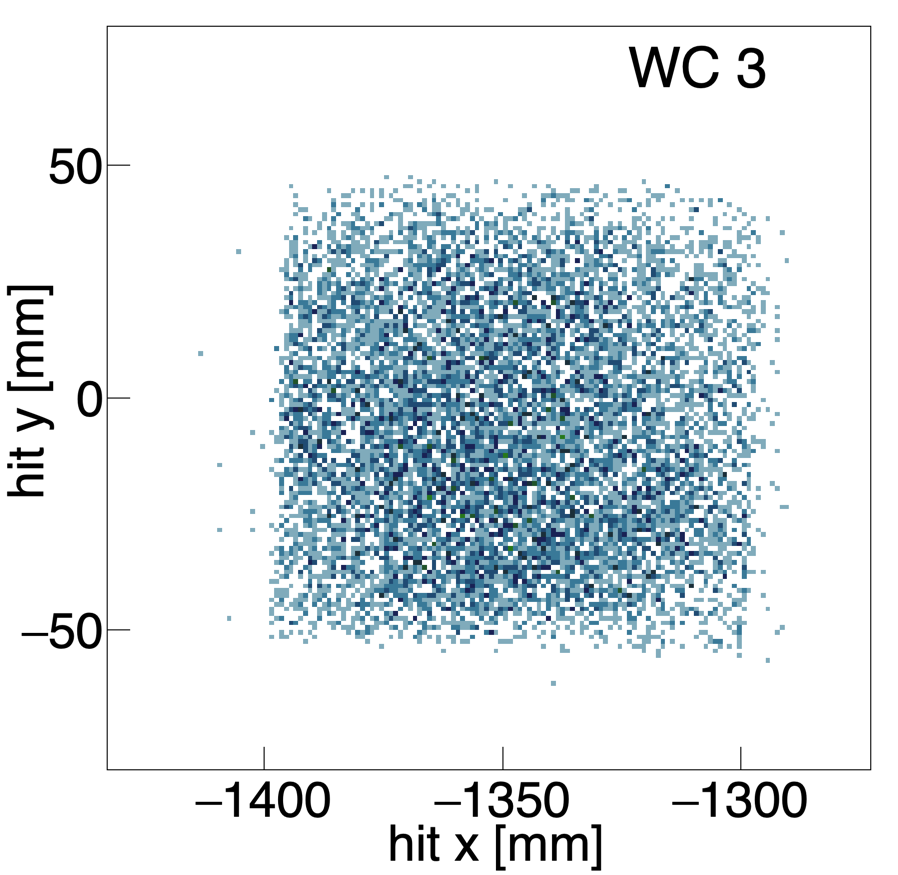
\includegraphics[width=\textwidth]{wcn_xy3_pol0_period4_miss0.png}
            \caption{WC3, P3}
            \label{fig_wc3_p3}
            \end{subfigure}
            \hfill    
             \begin{subfigure}[b]{0.23\textwidth}
            \centering
            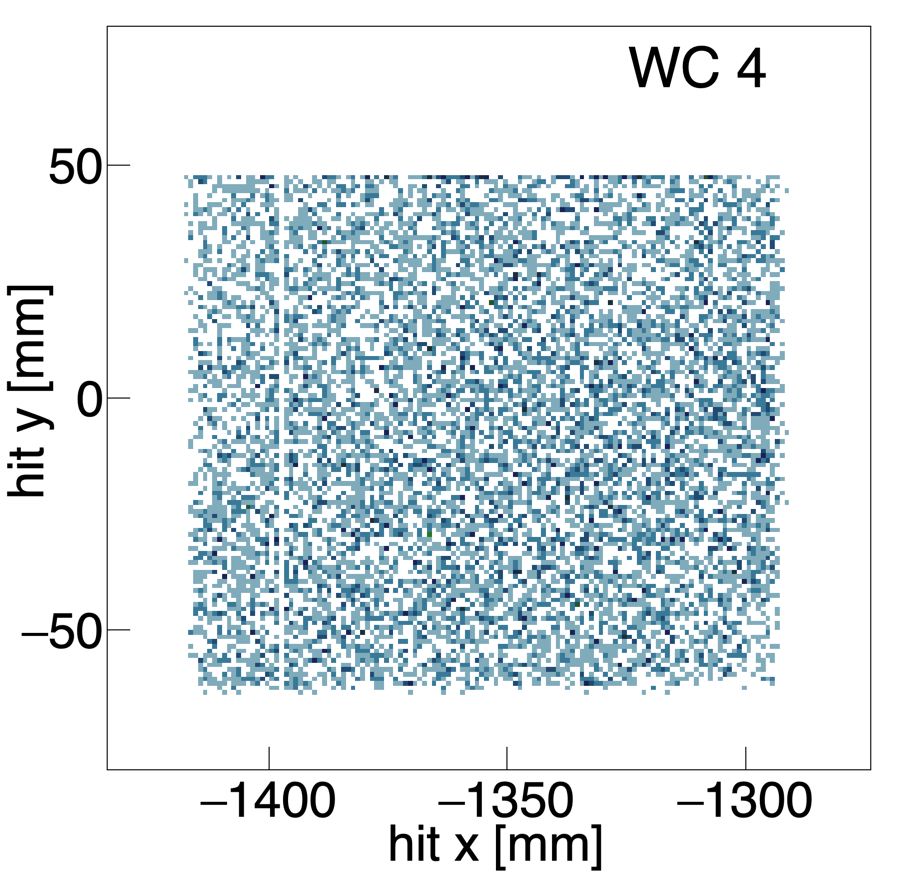
\includegraphics[width=\textwidth]{wcn_xy4_pol0_period4_miss0.png}
            \caption{WC4, P4, Negative}
            \label{fig_wc4_p3}
            \end{subfigure}
            \hfill
   %p4 positive
            \begin{subfigure}[b]{0.23\textwidth}
            \centering
            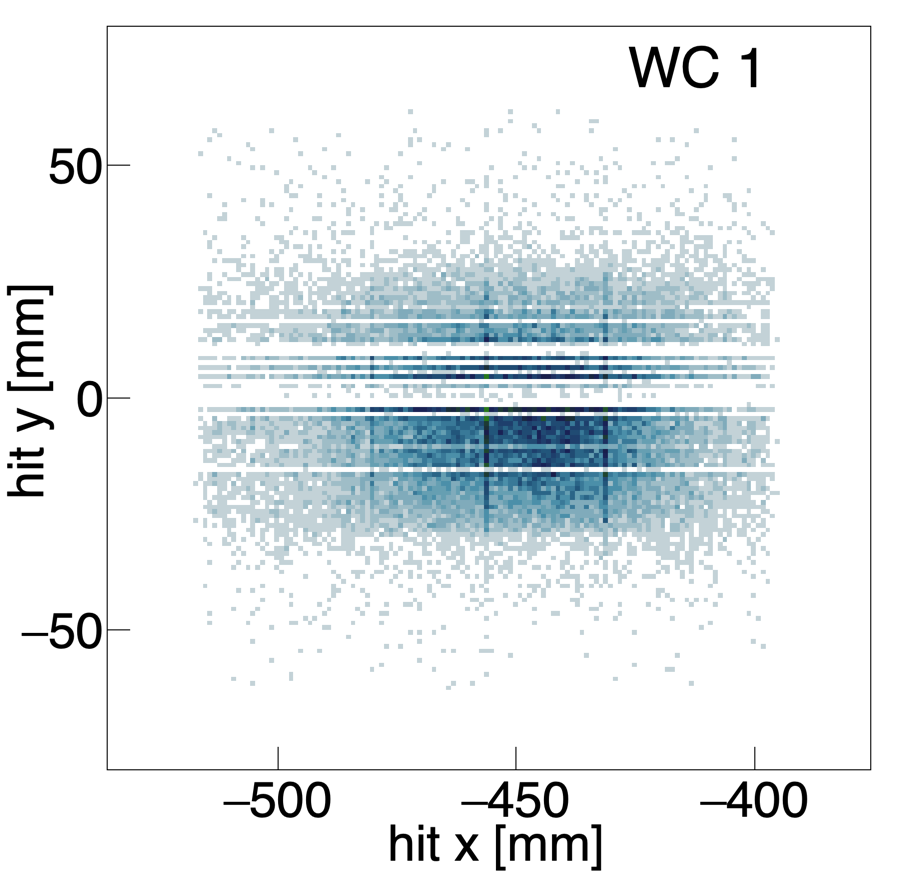
\includegraphics[width=\textwidth]{wcn_xy1_pol1_period4_miss0.png}
            \caption{WC1, P4}
            \label{fig_wc1_p4}
            \end{subfigure}
            \hfill             
             \begin{subfigure}[b]{0.23\textwidth}
            \centering
            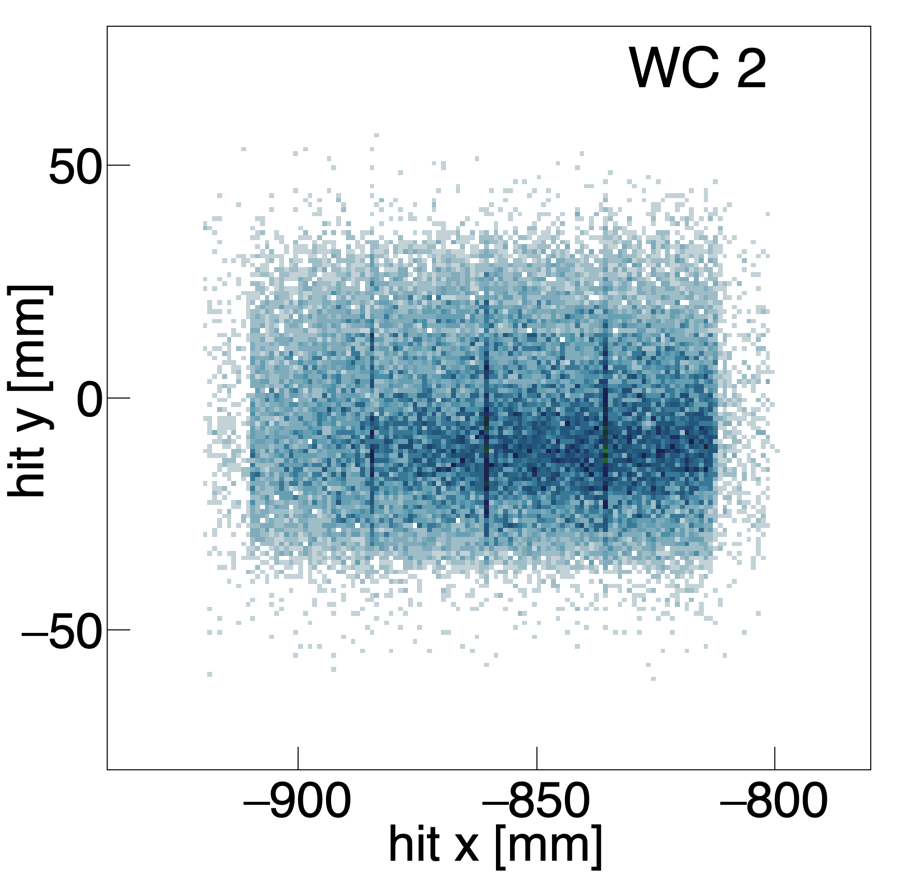
\includegraphics[width=\textwidth]{wcn_xy2_pol1_period4_miss0.png}
            \caption{WC2, P4}
            \label{fig_wc2_p4}
            \end{subfigure}
            \hfill 
              \begin{subfigure}[b]{0.23\textwidth}
            \centering
            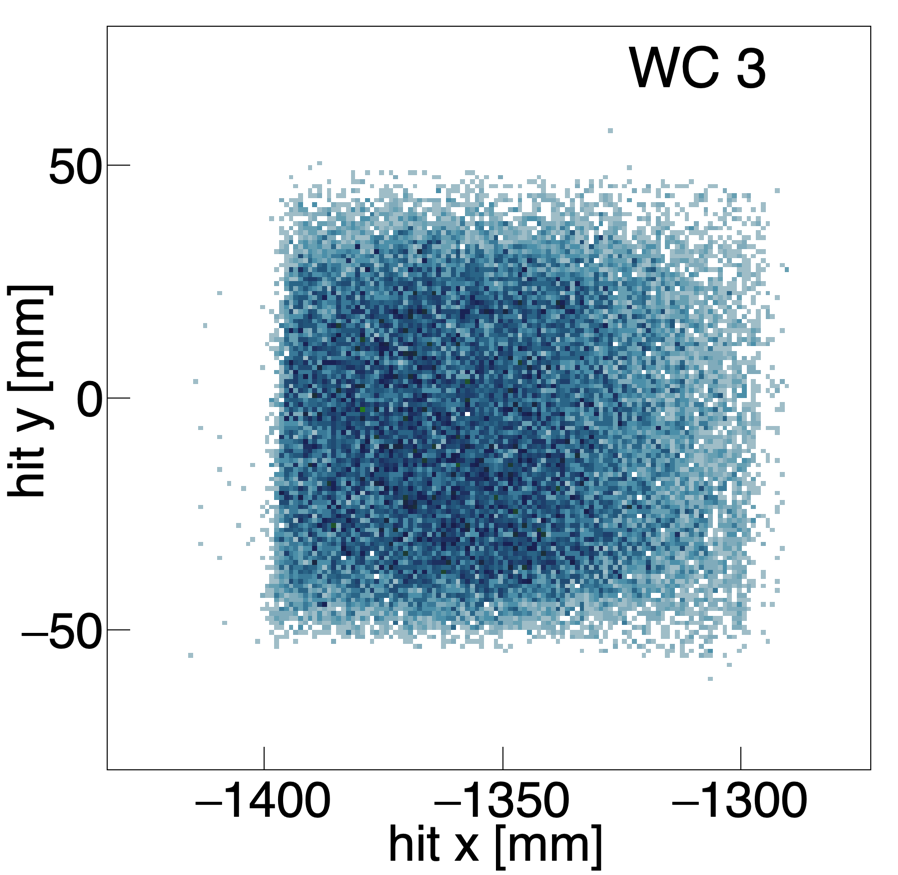
\includegraphics[width=\textwidth]{wcn_xy3_pol1_period4_miss0.png}
            \caption{WC3, P4}
            \label{fig_wc3_p4}
            \end{subfigure}
            \hfill    
             \begin{subfigure}[b]{0.23\textwidth}
            \centering
            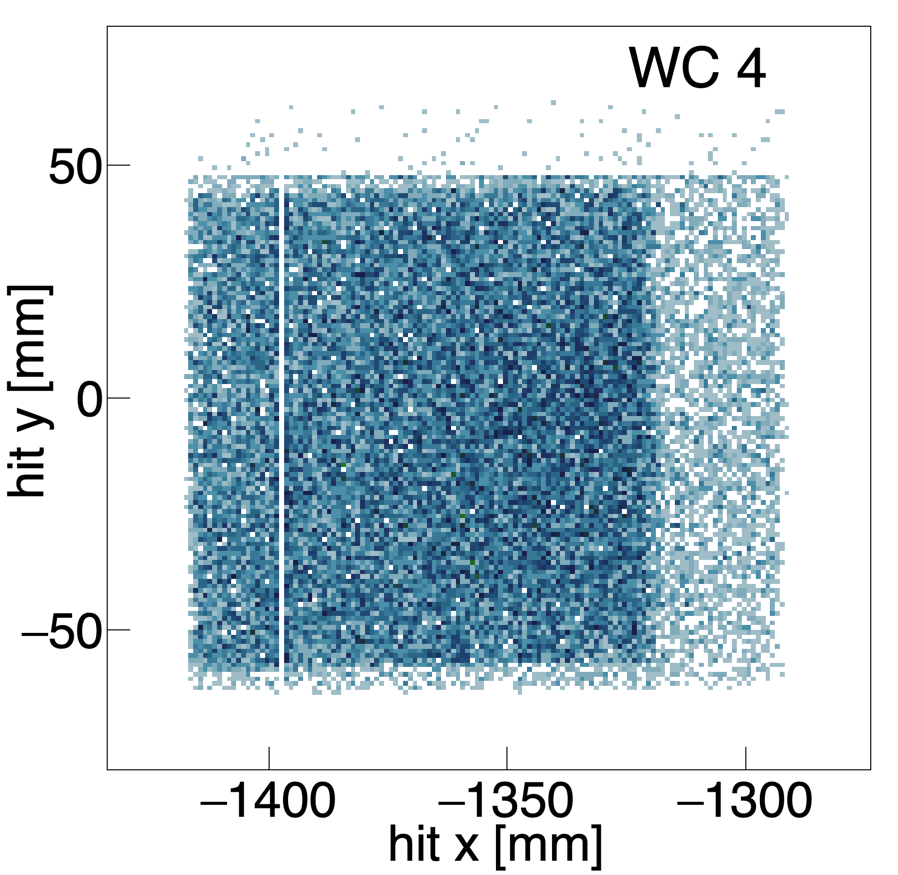
\includegraphics[width=\textwidth]{wcn_xy4_pol1_period4_miss0.png}
            \caption{WC4, P4}
            \label{fig_wc4_p4}
            \end{subfigure}
            \hfill
   \caption[short]{The WCTrack best hit position in each of the four wire chambers, in period 4, divided by polarity.}
   \label{fig_xyhitspol}
  \end{figure}
  
  
  
\newpage

\subsection{The rotation of the magnet}

Figure~\ref{fig_magnet} shows a sketch of a track passing through the magnetic field. The magnet is rotated about its center, contrary to what is shown in the technical drawings Figures~\ref{fig_td1} and ~\ref{fig_td2} . Figure~\ref{fig_xymag} show the entry point in x,y in the magnet's frame of the upstream track. 

\begin{figure}[h]	   
 \centering
        	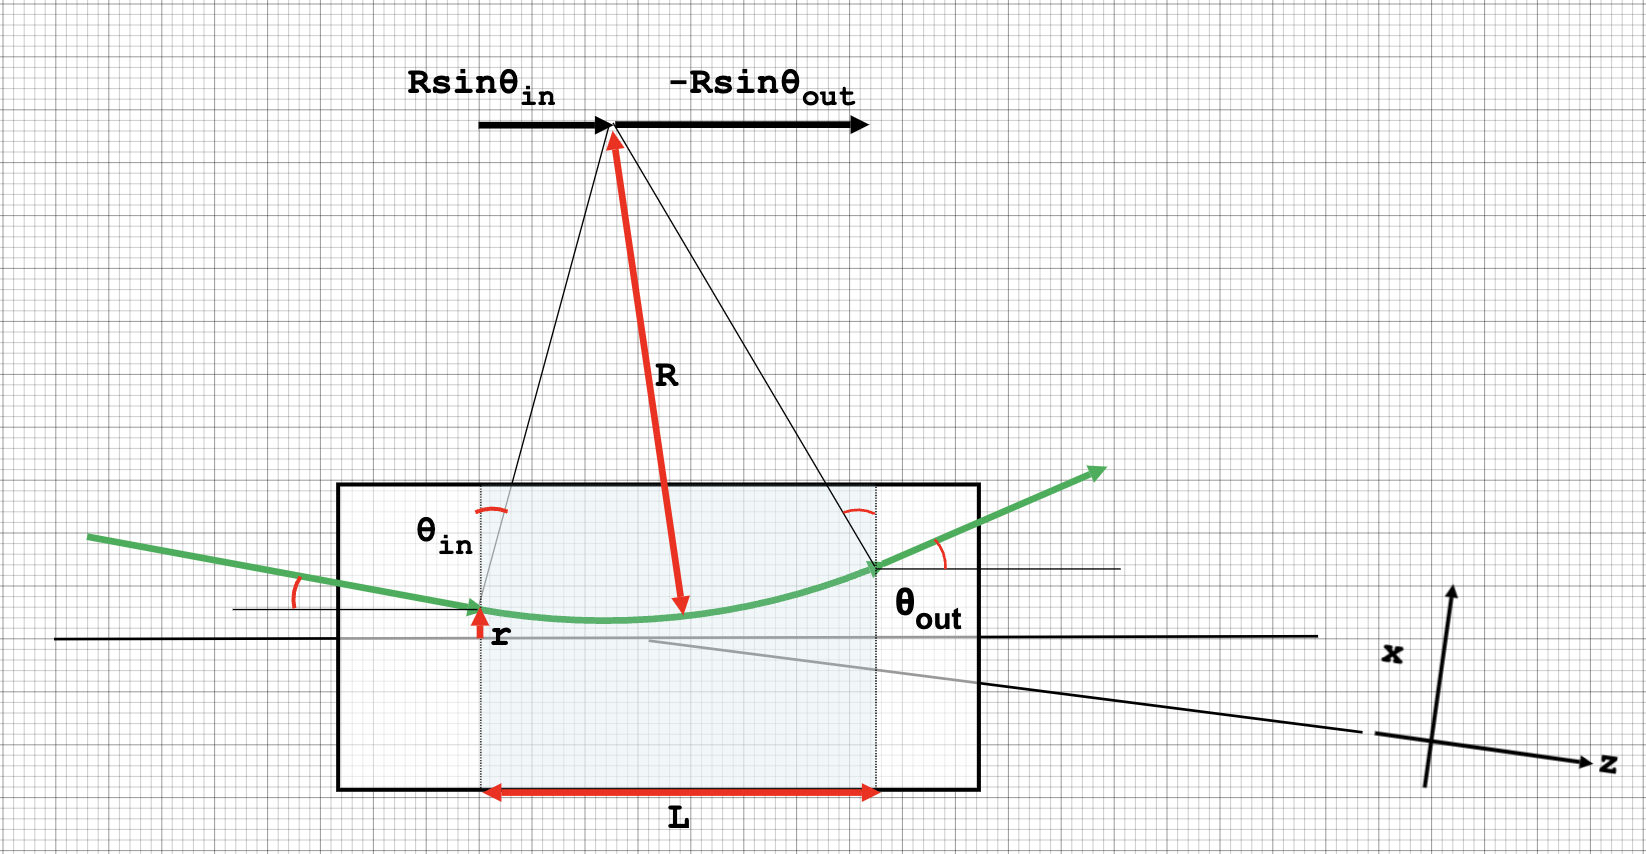
\includegraphics[scale=0.5]{magnet-detail.png}	 
   \caption[short]{Magnet details.}
   \label{fig_magnet}
  \end{figure}
  
  \begin{figure}[h]	   
 \centering
        	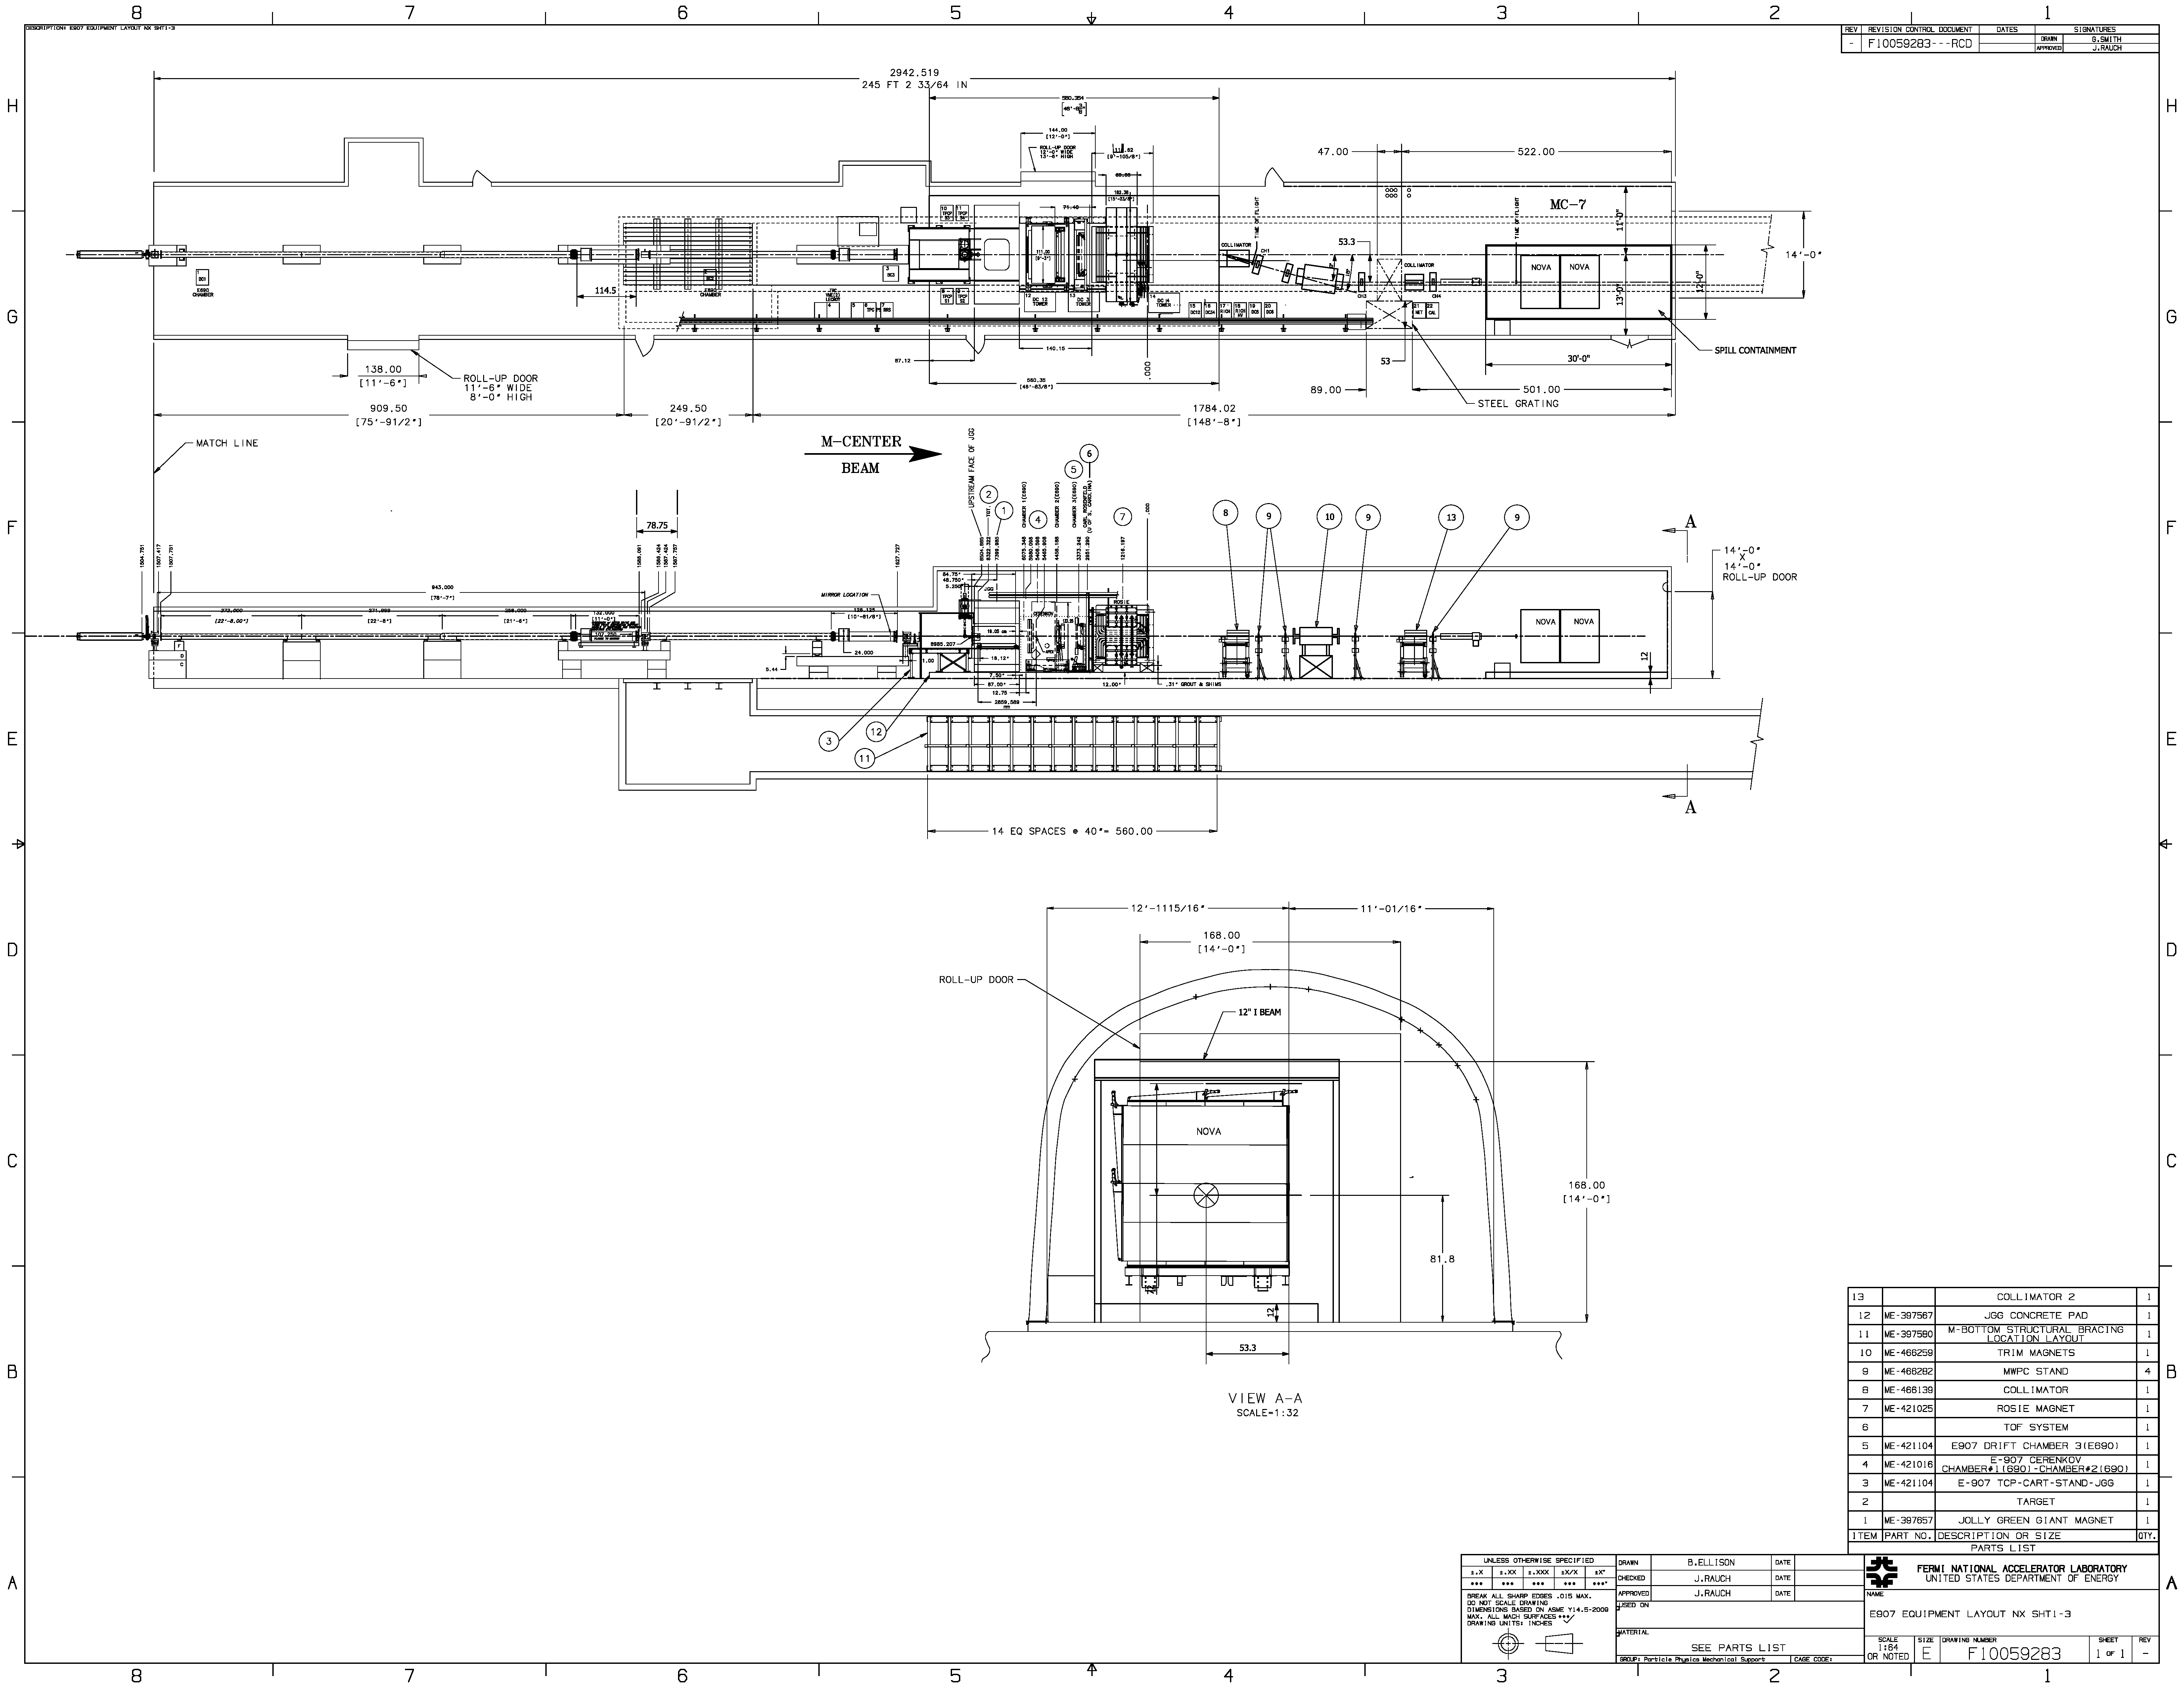
\includegraphics[scale=0.1]{ftbf_drawing.april_2018.pdf}	 
   \caption[short]{Technical drawing made before the decision to rotate the magnet around its center rather than its front face center.}
   \label{fig_td1}
  \end{figure}
  
    \begin{figure}[h]	   
 \centering
        	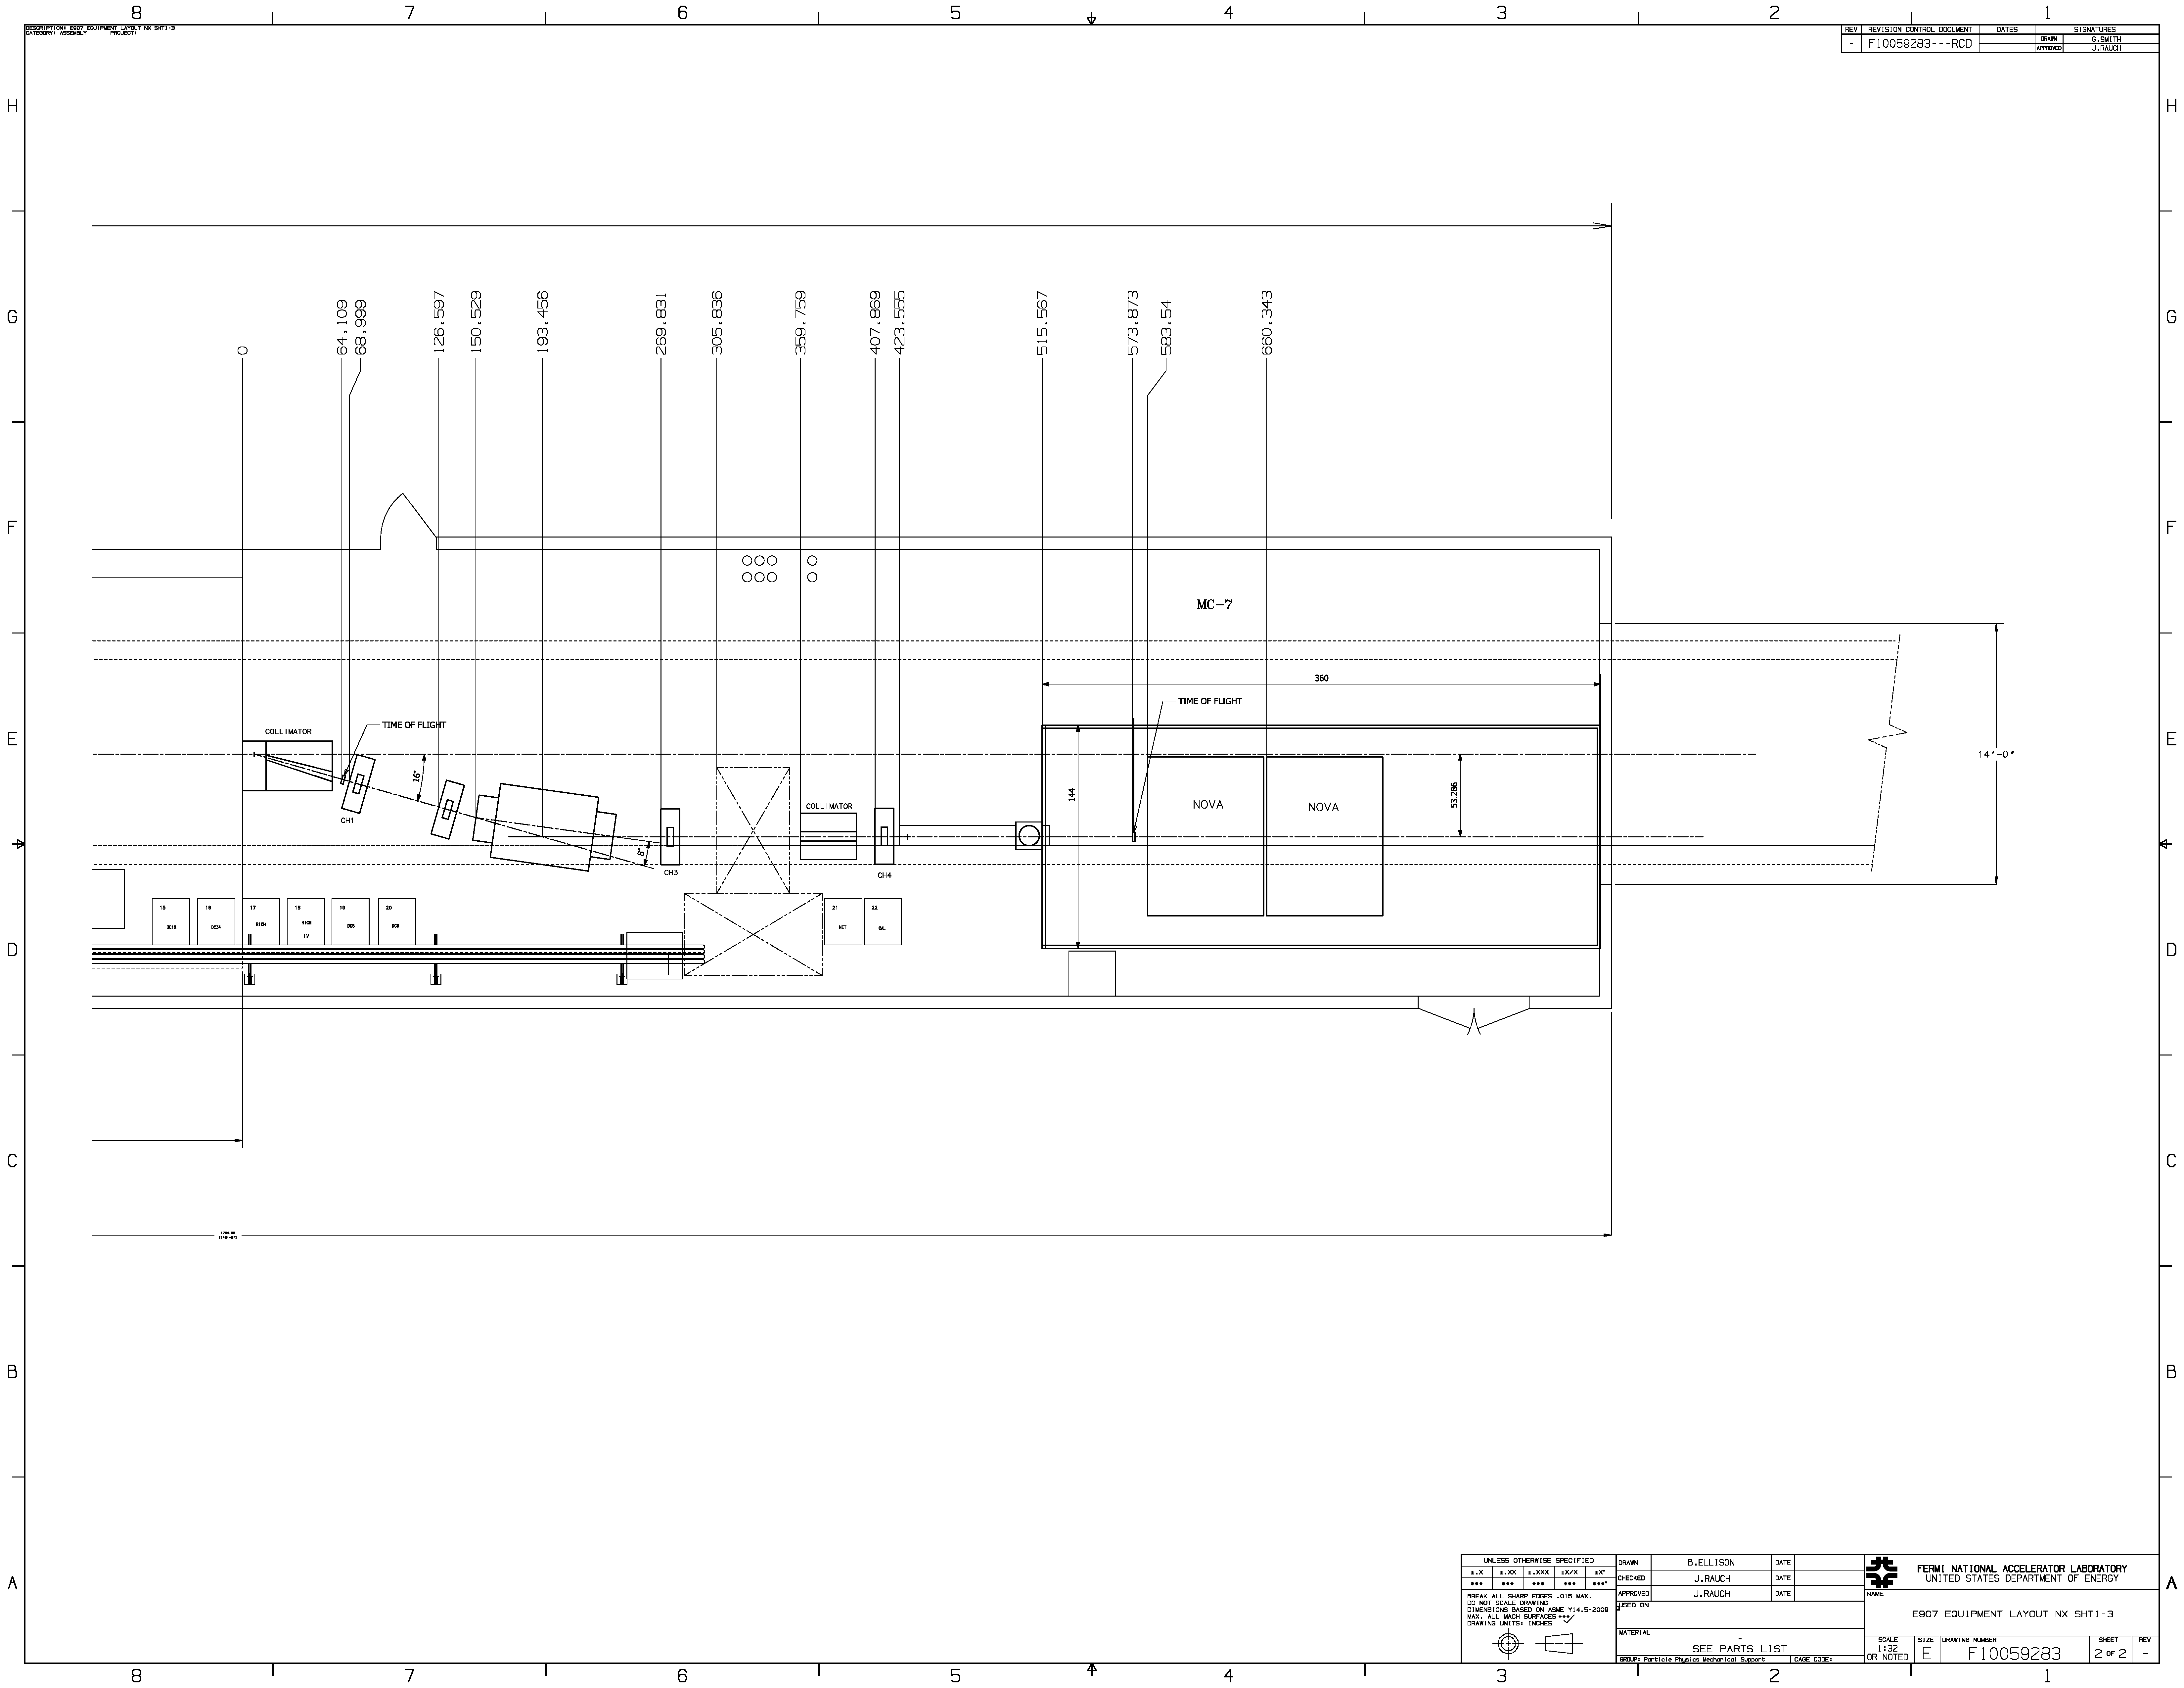
\includegraphics[scale=0.1]{gsmith_F10059283.may_2018.pdf}	 
   \caption[short]{Technical drawing made before the decision to rotate the magnet around its center rather than its front face center.}
   \label{fig_td2}
  \end{figure}
  
  

       \begin{figure}[h]	   
            \centering
%   
%            \begin{subfigure}[b]{0.48\textwidth}
%            \centering
            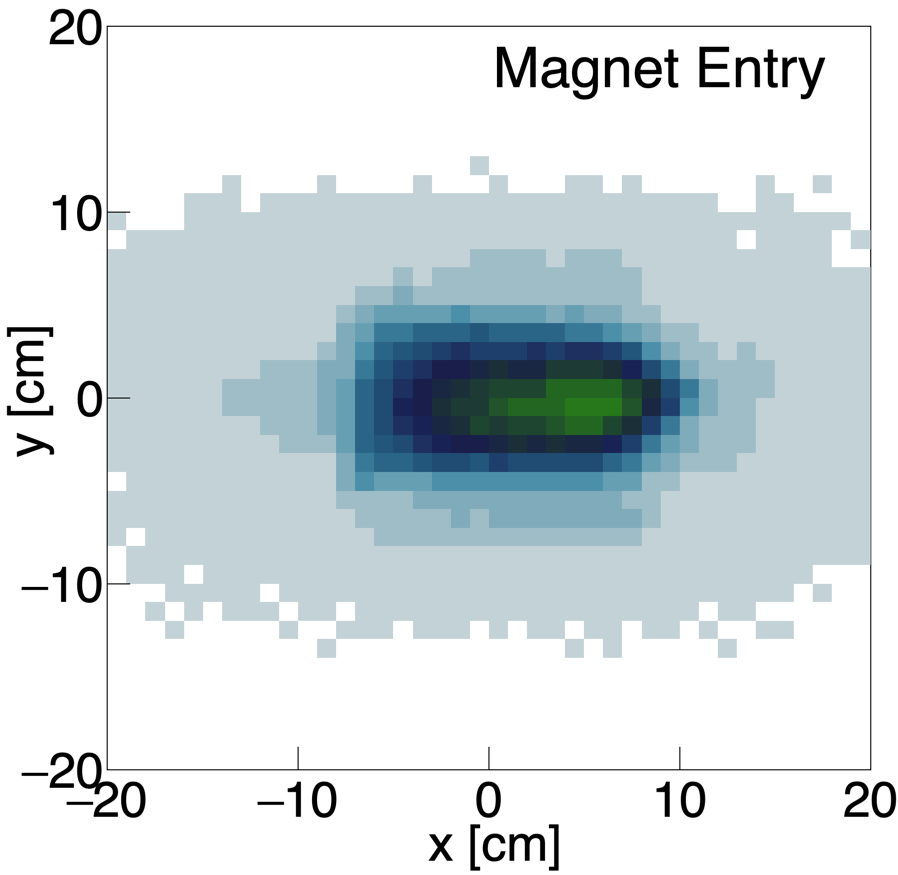
\includegraphics[scale=0.25]{wcn_mexy_pol-1_period234_cp0_range50.png}
             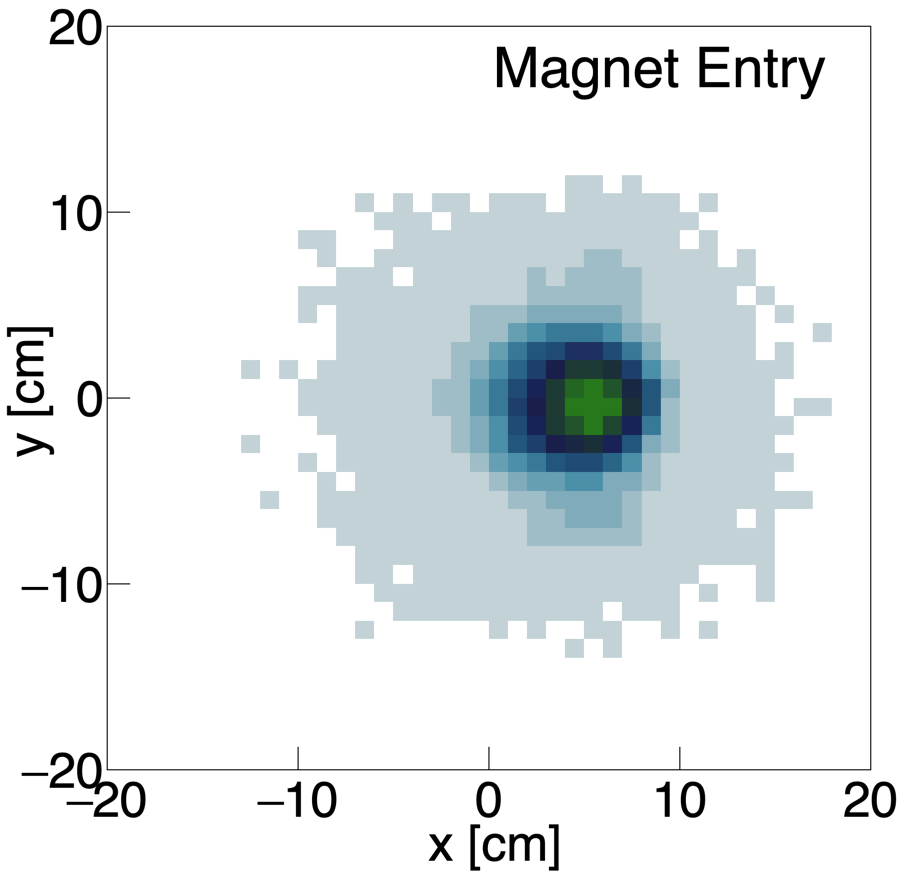
\includegraphics[scale=0.25]{wcn_mexy_pol-1_period234_cp1_range50.png}
%            \caption{$y=x$}
%            \label{fig:y equals x}
%            \end{subfigure}
%            \hfill             
%             \begin{subfigure}[b]{0.48\textwidth}
%            \centering
%            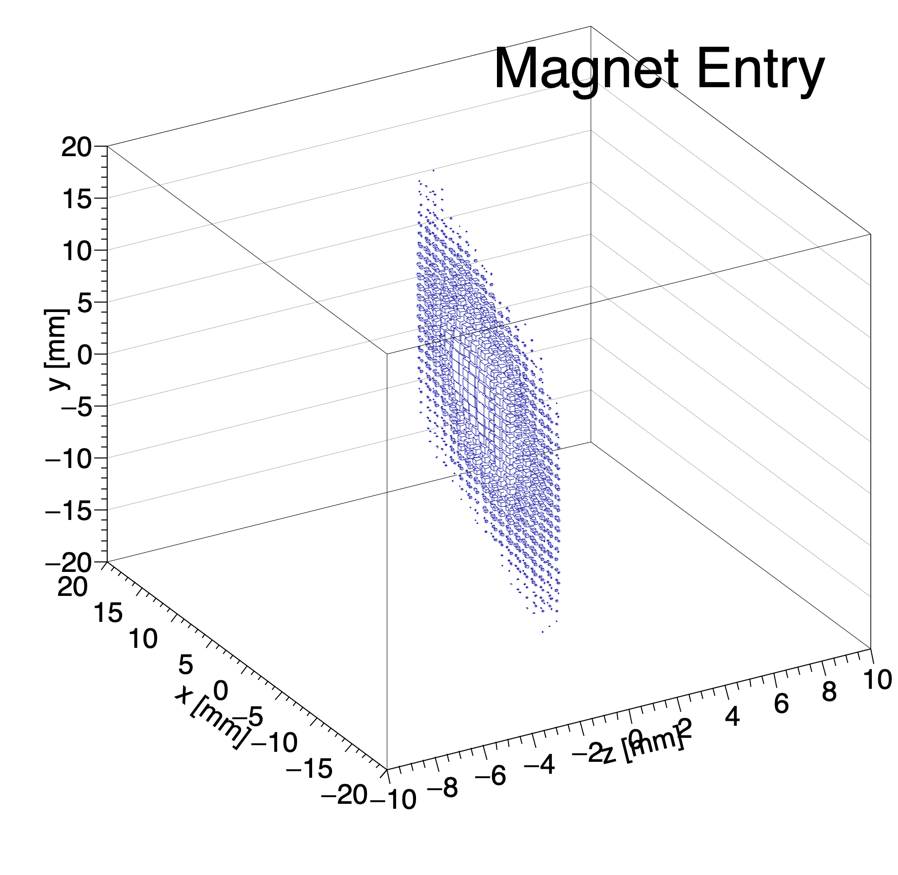
\includegraphics[width=\textwidth]{wcn_mexyz_pol-1_period234.png}
%            \caption{$y=x$}
%            \label{fig:y equals x}
%            \end{subfigure}
   \caption[short]{The x,y entry point of the upstream track to the magnetic field. On the left there is no constraint on the track having momentum consistent with the magnet current. On the right the track momentum must be within 10\% of the magnet current.}
   \label{fig_xymag}
  \end{figure}
  

  
  
  


 
